\chapter{Analysis strategies}

\begin{comment}
\section{Time Dependent \textit{CP} violation measurement}
The measurement of \textit{CP} violation in transitions of 
$B^0$ mesons to their common \textit{CP}
eigenstate $K_S^0 K_S^0 K_S^0$ requires the analysis of the time-dependent differential decay rates. The distribution of events based on the decay time difference $\Delta t$ and flavor is dependent on mixing induced and/or direct \textit{CP} parameters $\mathcal{S}$ and  $\mathcal{A}$. 

\begin{equation}
\mathcal{P}(\Delta t, q ) = 
\frac{e^{-|\Delta t|/\tau_{B^0}}}{4\tau_{B^0}}
\begin{Bmatrix}
1 + q \cdot 
\begin{bmatrix}
\mathcal{S}sin(\Delta M_d \Delta t) + 
\mathcal{A}cos(\Delta M_d \Delta t)
\end{bmatrix}
\end{Bmatrix}
\end{equation}

Here, same as discussed in Chapter 1, $\Delta M_d$ is the mass difference of two $B^0$ mass eigenstates, $\Delta t$ is the decay time difference of signal-side and tag-side $B^0$, namely $\Delta t = t_{CP} - t_{tag}$.  $\tau_B^0$ is the lifetime of $B^0$. And $q = + 1 (-1)$ is the indicator of flavor when tag-side meson is $B^0$ ($\bar{B^0}$). To a good aproximation using Eq(1.47), $\mathcal{A}$ is expected to be zero and $\mathcal{S} = -\text{sin}(2\phi_1)$, given the final states of $K_S^0 K_S^0 K_S^0$ corresponding to \textit{CP}-even ($n_f = + 1$). The previous result from Belle and Babar are shown in Fig 4-1. 

\begin{figure}
\centering 
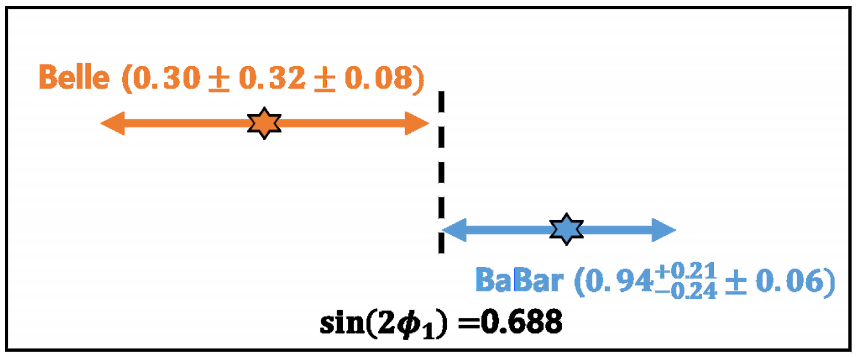
\includegraphics[height=5cm]{belle_babar_result}
\caption{The results of Belle (2007) and Babar on -sin(2$\phi_1$)}
\end{figure}
\end{comment}


\section{Data Sample and Event Selection}
\begin{comment}
The simulation data (MC) is taken from Belle II official MC campaign 13, named MC13. Both signal MC and generic MC are produced. In signal MC, one of the $B^0$ from $\Upsilon(4S)$ decays into final states 3$K_S^0$ then into 6 charged pions, while the other $B^0$ decays generically using all possible channels. In generic MC,  $B^0$ from  $\Upsilon(4S)$ all decay generically using all possible channels.
The signal MC sample is produced by EvtGen package with provided ``decay.dec" file that describes the required decay mode and branching fraction. As $K_S^0 \to \pi^0 \pi^0$ leads to large background with poor vertex quality, only the final states to 6 charged pions is used.
\end{comment}

As introduced in section 2.9, the branching fraction of $\mathcal{B}(B^0 \to K_S^0  K_S^0  K_S^0) = 6.0 \times 10^{-6}$. The simulation takes the $\Upsilon(4S)$ as the mother particle and generate its decay process to two scalar $B^0$ mesons with mixing. $B^0 \to K_S^0  K_S^0  K_S^0$ is simulated based on only the possible phase-space of kinematics that final states could have, which no $\it{CP}$ violation is assigned for $\mathcal{S}$(sin2$\phi_1$) and $\mathcal{A}$ in both signal and generic MC.

\subsection{$K_S^0$ Selection}
$K_S^0$ reconstruction is first reconstructed by the cut-based reconstruction which contains a large fraction of fake candidates, as discussed in chapter 3. In addition, a momentum cut on $K_S^0$ is used considering distribution in $B^0 \to K_S^0  K_S^0  K_S^0$. Only the $K_S^0$ candidates with momentum larger than 0.05 GeV are selected, as shown in Figure \ref{fig:ks-p}. 
\begin{figure}[ht]
	\centering
	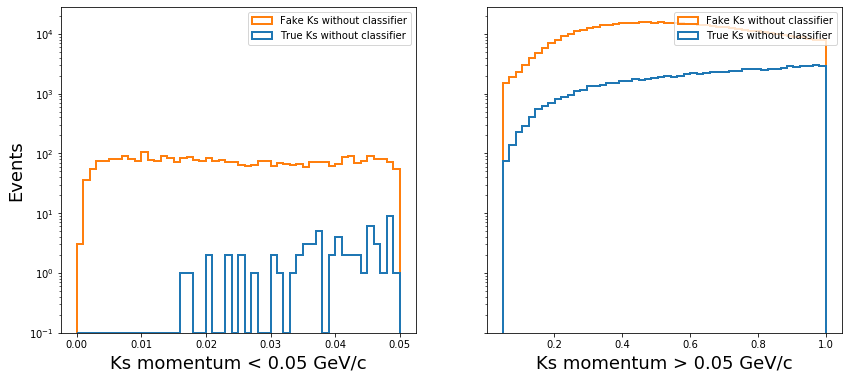
\includegraphics[height=6.5cm]{ks-p}
	\caption{The distribution of $K_S^0$ momentum. Candidates smaller than 0.05GeV/c are rejected. (Both plots shares the same y-axis scale on the left side.)}
	\label{fig:ks-p}
\end{figure}
Next, the vertex fit of $K_S^0$ is performed using \textit{TreeFit} package\cite{refId0}. Using fitted $K_S^0$ momentum and energy, fitted invariant mass is different from the one obtained directly using daughters' 4-vector. This quantity often receives impact of the measurement uncertainties. If we check out the distribution of fitted invariant mass based on daughters' SVD hits as section 3.1 discussed, \textit{SVD00} $K_S^0$ shows a large dispersion from the central region of the distribution of invariant mass after vertex fit, while \textit{SVD11} $K_S^0$ shows a small dispersion as shown in Figure \ref{fig:invm1}. Therefore, considering the $K_S^0$ candidates with different SVD hits, see Figure \ref{fig:ks-r-svdxx} and Table \ref{tab:svdxx}, reflecting the different tracking quality of daughter $\pi^{\pm}$, the different cut on invariant mass M$_{\pi^+\pi^-}$ after vertex fit is applied depending on the SVD hits number of pion tracks. As shown in Figure \ref{fig:invm}, the sideband regions where fake $K_S^0$ is much higher than true $K_S^0$ are excluded. The cut windows are listed in Table \ref{tab:ks_invm}. This improves the reconstruction purity.

\begin{figure}[htpb]
\centering
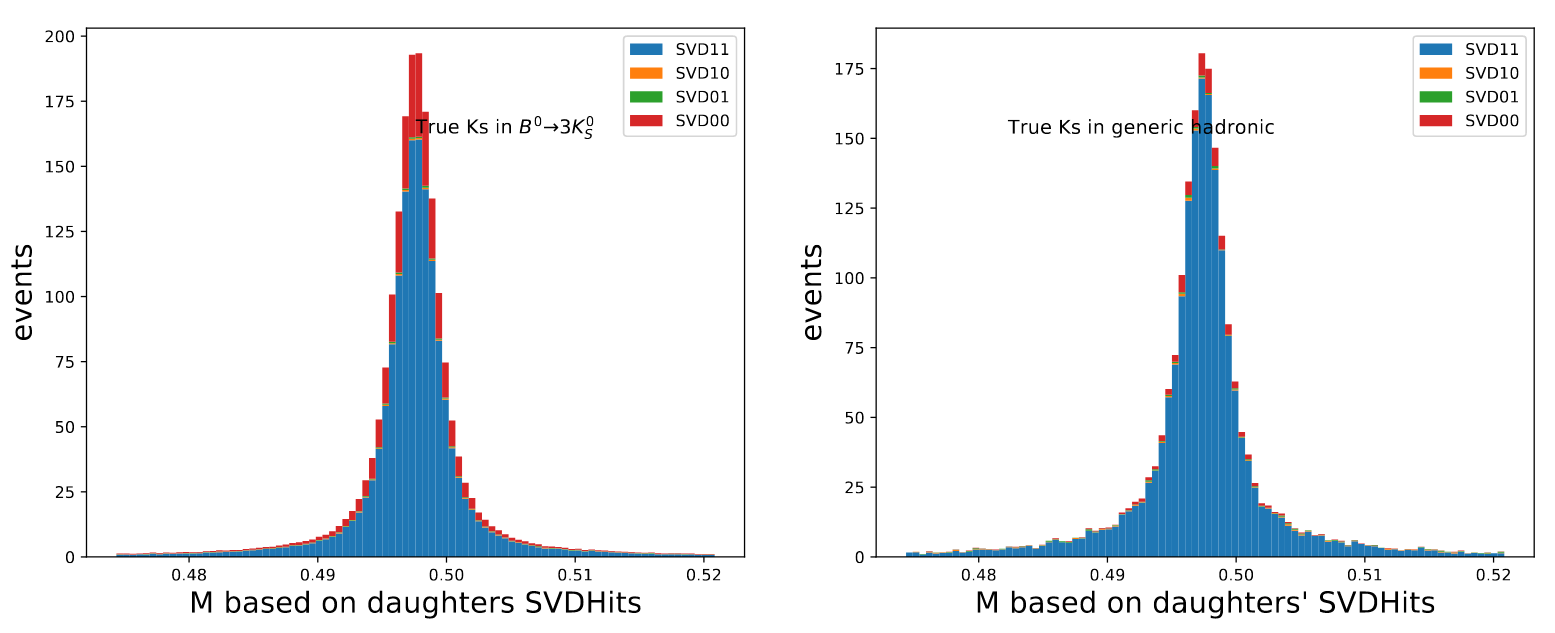
\includegraphics[width=0.7\linewidth]{m-before-fit}
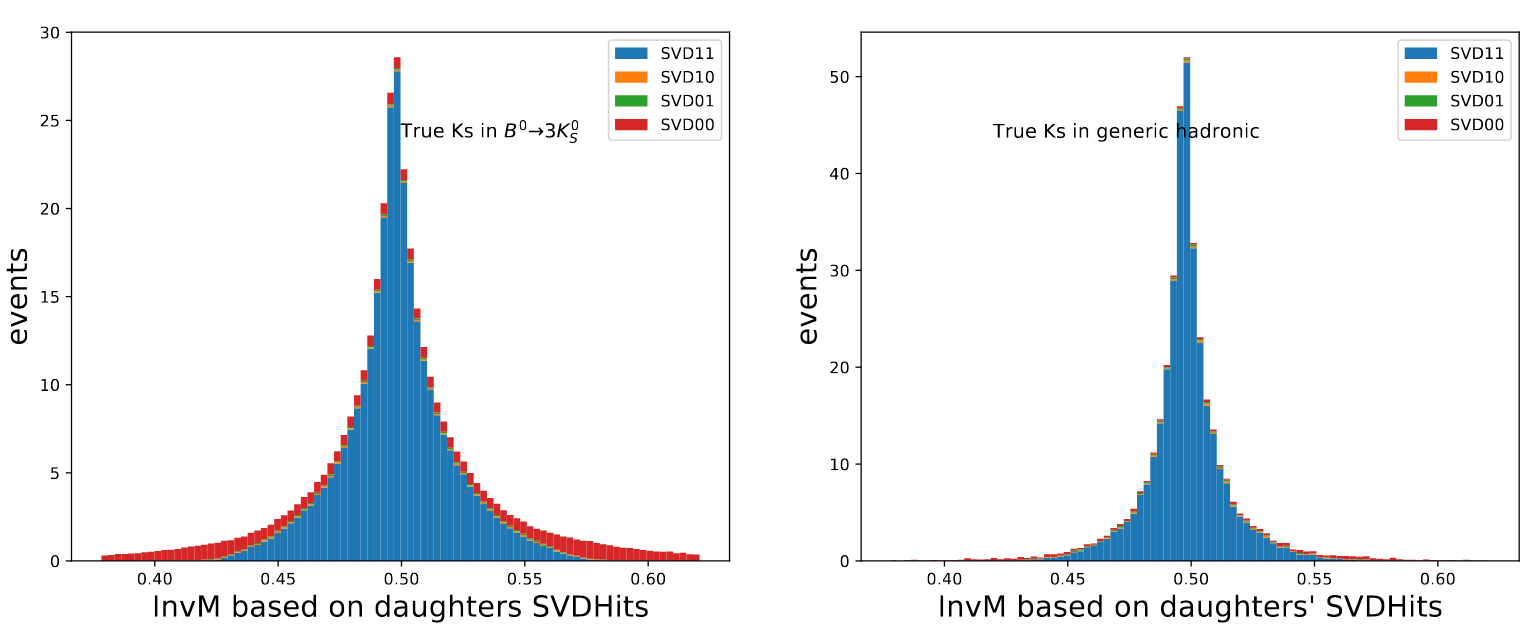
\includegraphics[width=0.7\linewidth]{m-after-fit}
\caption{(Top two plots)The invariant mass from daughters' 4-vector, the left is $B^0 \to K_S^0  K_S^0  K_S^0$  signal MC and the right is generic MC;
(bottom two plots)The invariant mass after vertex fit, the left is $B^0 \to K_S^0  K_S^0  K_S^0$  signal MC and the right is generic MC;
In both cases, the red shows the clear dispersion on \textit{SVD00} type $K_S^0$.}
\label{fig:invm1}
\end{figure}
 
In summary, $K_S^0$ are first reconstructed using BASF2 standard library with all converged vertex fit candidates are kept using \textit{TreeFit}. Then we reject $K_S^0$ candidates with momentum smaller than 0.05 GeV/c. After this, tuned cuts on invariant mass after vertex fit for each $K_S^0$ based on their SVD hits of pions are applied according to Table \ref{tab:ks_invm}. 
Eventually, only $K_S^0$ with ``FBDT\_Ks" larger than 0.74 are kept based on Figure \ref{fig:ks_fom}.
 
\begin{table}[h]
	\centering 
	\begin{tabular}{|c|c|c|c|c|} 
		\hline
		$K_S^0$ type & SVD11 & SVD10 & SVD01  & SVD00  \\
		\hline
		M$_{\pi^+\pi^-}$ window (GeV) & (0.45,0.55) & (0.38,0.7)  & (0.38,0.7)  & (0.3,0.7) \\
		\hline
	\end{tabular}
\caption{Invariant mass cut window after vertex fit for $K_S^0$ based on Figure \ref{fig:invm}.}
\label{tab:ks_invm}
\end{table}

\begin{figure}[htpb]
	\centering
	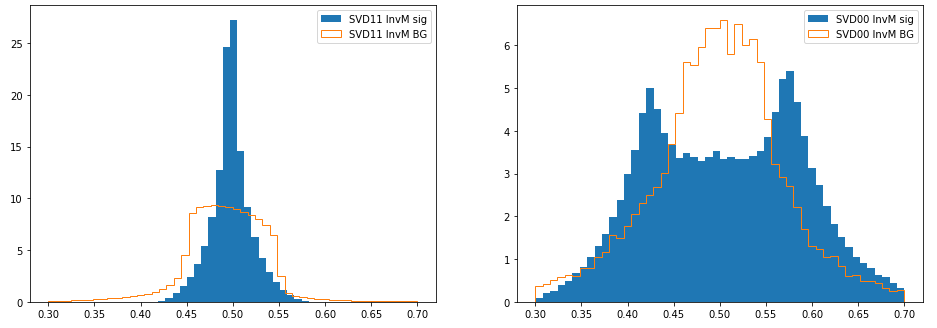
\includegraphics[width=0.7\linewidth]{invm1}
	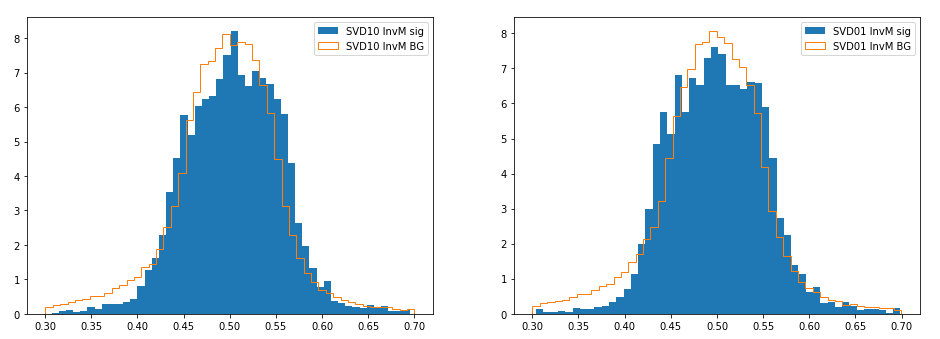
\includegraphics[width=0.7\linewidth]{invm2}
	\caption{Invariant mass after vertex fit of $K_S^0$, the sideband is excluded in each distribution to further reject fake $K_S^0$}
	\label{fig:invm}
\end{figure}

\subsection{$B^0$  Reconstruction}
\begin{comment}
The energy of $B^0$ should be exactly the half of the energy in CMS frame, so replacing the energy of $B^0$ with half of the beam energy in the calculation of invariant mass of reconstructed $B^0$, $M_{bc}$ can be expressed as: 

\begin{equation}
M_{bc} = \sqrt{(s/2+\boldsymbol{p_B p_0})^2/{E_0^2}-\boldsymbol{p_B^2}} 
\end{equation}
where $E_0$ and $\boldsymbol{p_0}$ are the energy and momentum of CMS in the lab frame. $s$ is the invariant mass of the system. By the definition of $M_{bc}$ is clear that it's independent from the mass hypotheses of reconstructed particle. On the contrary, $\Delta{E}$ can be presented as:
\begin{equation}
\Delta{E} = (2q_B q_0-s)/2\sqrt{s}
\end{equation}
where $q_B$ and $q_0$ are the 4-vector of $B^0$ and CMS in lab frame. \cite{Bevan_2014}. $\Delta{E}$ receives sizable contribution from beam energy dispersion but is generally dominated by the reconstruction resolution of detector. It's expected to be centered at zero  And it's affected by the invariant mass of particle. These two variables are much more independent than $p_B$ and $E_B$, so combination of them can be used as a 2-D distribution which yields correctly reconstructed $B^0$.

 The reconstruction are conducted on both samples with or without beam background, to evaluate the influence of beam background. As discussed in previous section, $K_S^0$ efficiency is depending on the CDC tracking especially for the long-lived ones. Yet CDC is suffering from the high beam background level at targeted luminosity of SuperKEKB. Even though at current stage, the MC samples are generated with early phase 3 geometry and luminosity, such effect might be trivial, the comparison of sensitivity among them is still worth noticing. The event selection of using different $K_S^0$ criteria are included as well.
 
\end{comment}
By combining three $K_S^0$ particles from selected dataset, we can reconstruct $B^0$. The beam-constraint mass $M_{bc}$ and energy difference $\Delta E$ are used to extract signal, as defined in Equation \ref{eq:mbc} and \ref{eq:dE}, respectively. 
 The $B^0$ candidates with $M_{bc} > 5.2$ GeV and $|\Delta{E}| < 0.2$ GeV are requested. Then the vertex fit using \textit{TreeFit} is performed on each $B^0$ candidate and only $B^0$ with converged vertex fit result is kept. When multiple $B^0$ candidates show up in a single event, the best candidates selection (BCS) is performed by ranking their vertex fit quality. Since the BCS is based on the vertexing quality that might introduce bias in the vertex positions for $\it{CP}$ fit, we check the distribution of the vertex $\chi_2$, as shown in Figure \ref{fig:b0dist} top right. The distribution of candidates number per event without BCS is shown in top left of Figure \ref{fig:b0dist} as well, showing a consistence between data and generic MC within 1$\sigma$. The distribution of candidates per event is in an agreement with the one from signal MC (bottom left of Figure \ref{fig:b0dist}). The 2D distribution of $M_{bc}$ and $\Delta E$ from $B^0 \to K_S^0  K_S^0  K_S^0$ signal MC is shown in Figure \ref{fig:b0dist}  bottom right.
 
 \begin{equation}\label{eq:mbc}
 M_{bc} = \sqrt{\frac{s}{4}-p^{*2}_B} 
 \end{equation}
 
 \begin{equation}\label{eq:dE}
 \Delta E = E^*_B - \frac{\sqrt{s}}{2}
 \end{equation}
 
\begin{figure}[H]
	\begin{minipage}[b]{0.5\linewidth}
		\centering 
		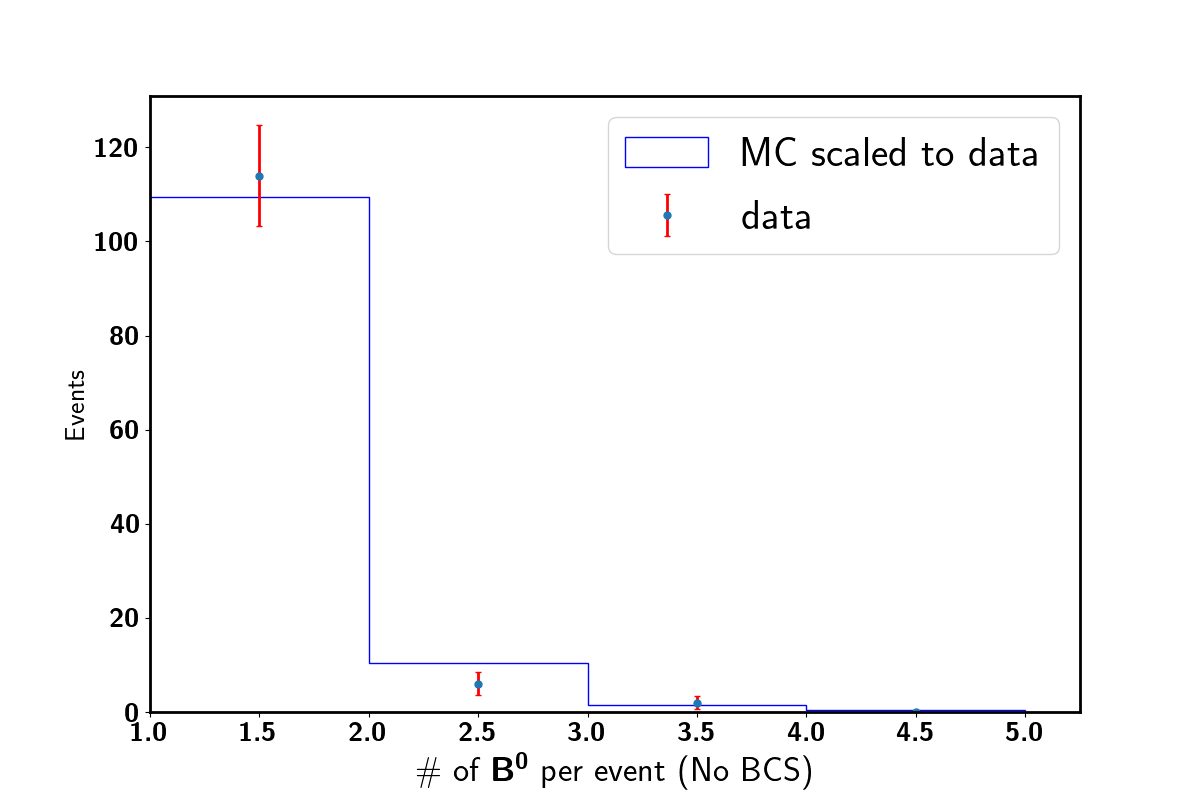
\includegraphics[height=6cm]{figures/best_ncands_noBCS}
		
	\end{minipage}
	\begin{minipage}[b]{0.5\linewidth}
		\centering 
		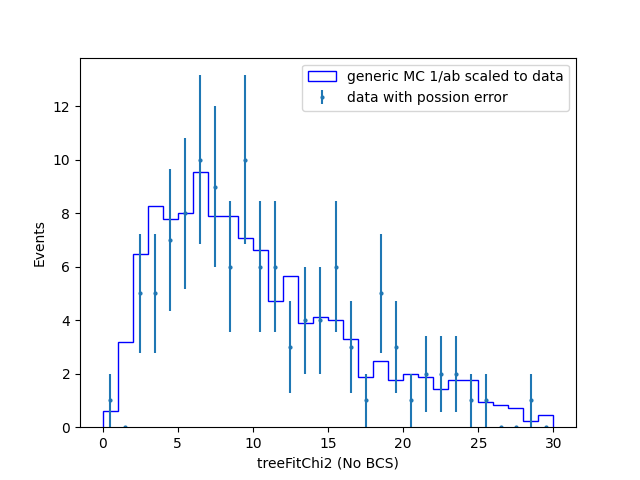
\includegraphics[height=6cm]{figures/best_treeFitChi2_noBCS}
		
	\end{minipage}
	\begin{minipage}[b]{0.5\linewidth}
		\centering 
		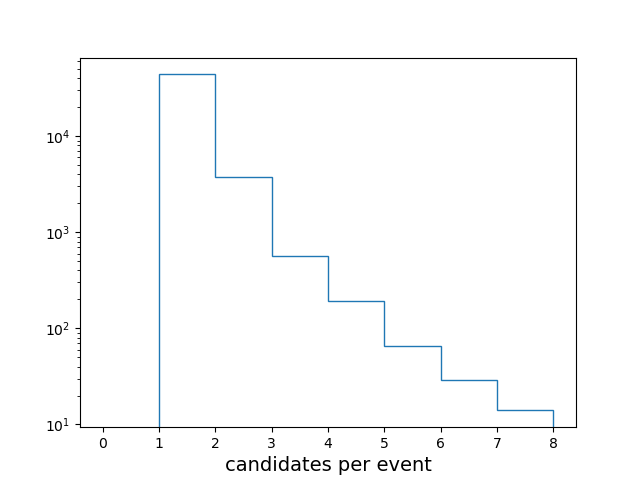
\includegraphics[height=6cm]{figures/best_cands}
		
	\end{minipage}
	\begin{minipage}[b]{0.5\linewidth}
		\centering 
		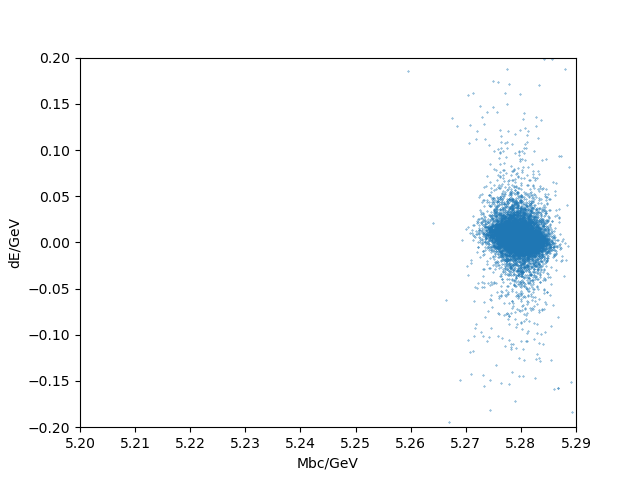
\includegraphics[height=6cm]{figures/hist_sig_MC_Mbc_dE}
		
	\end{minipage}
	
	\caption{Top left is the candidates per event in data and generic MC before the BCS. Top Right is the $\chi_2$ for data and generic MC before BCS. Bottom left is the number of candidates $B^0$ per event from signal MC. Bottom right is the 2D $M_{bc}$ and $\Delta E$ distribution from signal MC.}
	\label{fig:b0dist}
\end{figure}


% move to after CS
The summary of $B^0$ selections for is:
\begin{table}[H]
	\centering 
	\begin{tabular}{|c|c|c|c|c|c|c|c|} 
		\hline
		$B^0$  & $M_{bc}$/GeV& $\Delta E$/GeV & chiProb & Rank & FBDT\_CS & FBDT\_Ks\\
		\hline
		Selection & $> 5.20$ \& $< 5.29$  &  $ |\Delta E|< 0.2$ & $> 0.001$  & $=1$ & $>0.66$ & $>0.74$\\
		\hline
	\end{tabular}
	\caption{$B^0$ selection criteria}
\end{table}

The Table 4.4 shows that, given the newly developed $K_S^0$ selection, efficiency of $B^0$ reconstruction as well as purity is slight improved in Belle II compared to Belle.
\begin{table}[H]
	\centering
	\begin{tabular}{c|c|c|c|c}
		\hline
		event selection & efficiency & purity  & $f_{MB}$  & BCS \\
		\hline
		\hline
		Belle Standard & 35\%(33\%) & 96\%(99\%) & 6\%(6\%) & 83\%(96\%)\\
		\hline 
		Belle II (BG1) & 36\%(34\%) & 96\%(98\%) & (4\%)(4\%) & 95\%(96\%)\\
		\hline
		Belle II (BG0) & 40\%(36\%) & 96\%(99\%) & (3\%)(3\%) & 97\%(97\%)\\
		\hline
	\end{tabular}
	\caption{The efficiency is defined by the fraction of best candidates among the MC input number. Purity is the fraction of true $B^0$ in best candidates. $f_{MB}$ stands for multiple $B^0$ events fraction in signal. BCS is the fraction of best candidates being a true signal. All values in the parenthesis are calculated in $| M_{bc} |- 5.28 < 0.1$ and $|\Delta E| < 0.1$, or called ``signal region" where efficiency is lower but purity is higher. }
\end{table}
\subsection{Continuum Suppression}
The production cross-section of $B\bar{B}$ from $\Upsilon{(4S)}$ receives a sizable contribution from other flavor of quarks other than b quark. This calls a demand to distinguish a specific $B\bar{B}$ decay events from combinatorial background from $e^+e^- \to q\bar{q}$, so called continuum suppression (CS). The rejection is essential because it's the dominated background.  In the case of $b \to s$ charmless decay like $B^0 \to K_S^0  K_S^0  K_S^0$, the number of continuum background can exceed the signals by a few orders of magnitudes without suppression. In a $B\bar{B}$ event, two mesons are produced almost at rest in the CMS frame since the resonance state $\Upsilon(4S)$ is  just slightly lighter than beam energy. As a result	, decay products are emitted more isotopically, compared to continuum background. The ARGUS and CLEO collaboration\cite{Bevan_2014} developed a set of variables to suppress the continuum, which has also been implemented into BASF2 framework. 

CLEO cones momentum can be presented as Equation \ref{eq:ln}, where $ p_i $ is momentum of i-th particle in Rest-Of-Event (ROE) particles in a event except for the ones used to reconstructed $\it{CP}$-side $B^0$, $\theta_i$ is angle against momentum thrust of reconstructed $\it{CP}$-side of \textit{B} meson.

\begin{equation}\label{eq:ln}
L_n = \sum_{i\in ROE}^{} p_i \times |cos\theta_i|
\end{equation}

Besides, the modified Super Fox-wolfram momentum named  KSFW momentum, are calculated in each event. The KSFW momentum are defined as shown in Equation \ref{eq:ksfw}. 
\begin{equation}\label{eq:ksfw}
KSFW = \sum_{l=0}^{4}( R_l^{so} + R_l^{oo}) + \gamma \sum_{n=1}^{N_t}|P(t)_n|
\end{equation}
where the first term is shown in Equation \ref{eq:rlso}.
\begin{equation}\label{eq:rlso}
R_l^{so} = \frac{\alpha_{cl}H_{cl}^{so} +
				\alpha_{nl}H_{nl}^{so}+
			\alpha_{ml}H_{ml}^{so}}{E^*_{beam}-\Delta E}
\end{equation}

when l is odd in Equation \ref{eq:rlso}: 
\begin{equation}
	H_{nl}^{so}=H_{ml}^{so}=0
\end{equation}
and $H_{cl}^{SO}$ is defined as shown in Equation \ref{eq:hclso}: 
\begin{equation}\label{eq:hclso}
	H_{cl}^{so} = \sum_i \sum_{jx}Q_i Q_{jx}|p_{jx}|P_l(cos\theta_{i,jx})
\end{equation}
\textit{i} runs over \textit{B} daughter particles and \textit{jx} for other particles in ROE. \textit{Q} is charge and $p_{jx}$ is momentum for each particle. $P_l(cos\theta_{i,jx})$ is the \textit{i}-th order Legendre polynomial of cosine of \textit{i} and \textit{jx}-th particles.
On the other hand, for \textit{l} is even, $H_{xl}^{SO}$ can be written in Equation \ref{eq:hxlso}.
\begin{equation}\label{eq:hxlso}
	H_{xl}^{so}=\sum_i \sum_{jx}|p_{jx}|P_l(cos\theta_{i,jx})
\end{equation}
The second term in Equation \ref{eq:ksfw}, when \textit{l} is odd, can be defined as Equation \ref{eq:roo}.
\begin{equation}\label{eq:roo}
	R^{oo}_l = \sum_j \sum_k \beta_l Q_j Q_k |p_j||p_k|P_l(cos\theta_j,k)
\end{equation}
\textit{j} and \textit{k} runs over ROE particles and others are same as Equation \ref{eq:hclso}.
For an even \textit{l}: 
\begin{equation}
	R^{oo}_l = \sum_j \sum_k \beta_l |p_j||p_k|P_l(cos\theta_j,k)
\end{equation}
$\beta$ is five Fisher coefficient to be determined. 
Using above definitions, we can form the possibility density functions for KSFW, cosine angle against \textit{B} meson thrust and $\Delta Z$ of two side vertices.  Then based on each event's variables' value, we can calculate a ratio $\mathcal{R}$ as Equation \ref{eq:Rcs}, where the likelihood $L$ of signal($L_S$) and background($L_B$) are obtained from the possibility density functions defined in Equation \ref{eq:Lsb}.
The $ \mathcal{R} $ is: 
\begin{equation}\label{eq:Rcs}
	\mathcal{R} = \frac{L_S}{L_S+L_B}
\end{equation}
\begin{equation}\label{eq:Lsb}
L_{S/B} = P(KSFW)_{S/B} \times P(cos\theta_B)_{S/B} \times P(\Delta Z)_{S/B}
\end{equation}
where \textit{P} is probability density function for signal and continuum, depending on the discriminating variables in the parentheses. For example, the distribution of a variable called $R_2$ shown in Figure \ref{fig:R2} where the possibility density function is different for signal and continuum events in generic MC.

\begin{figure}[H]
	\centering
	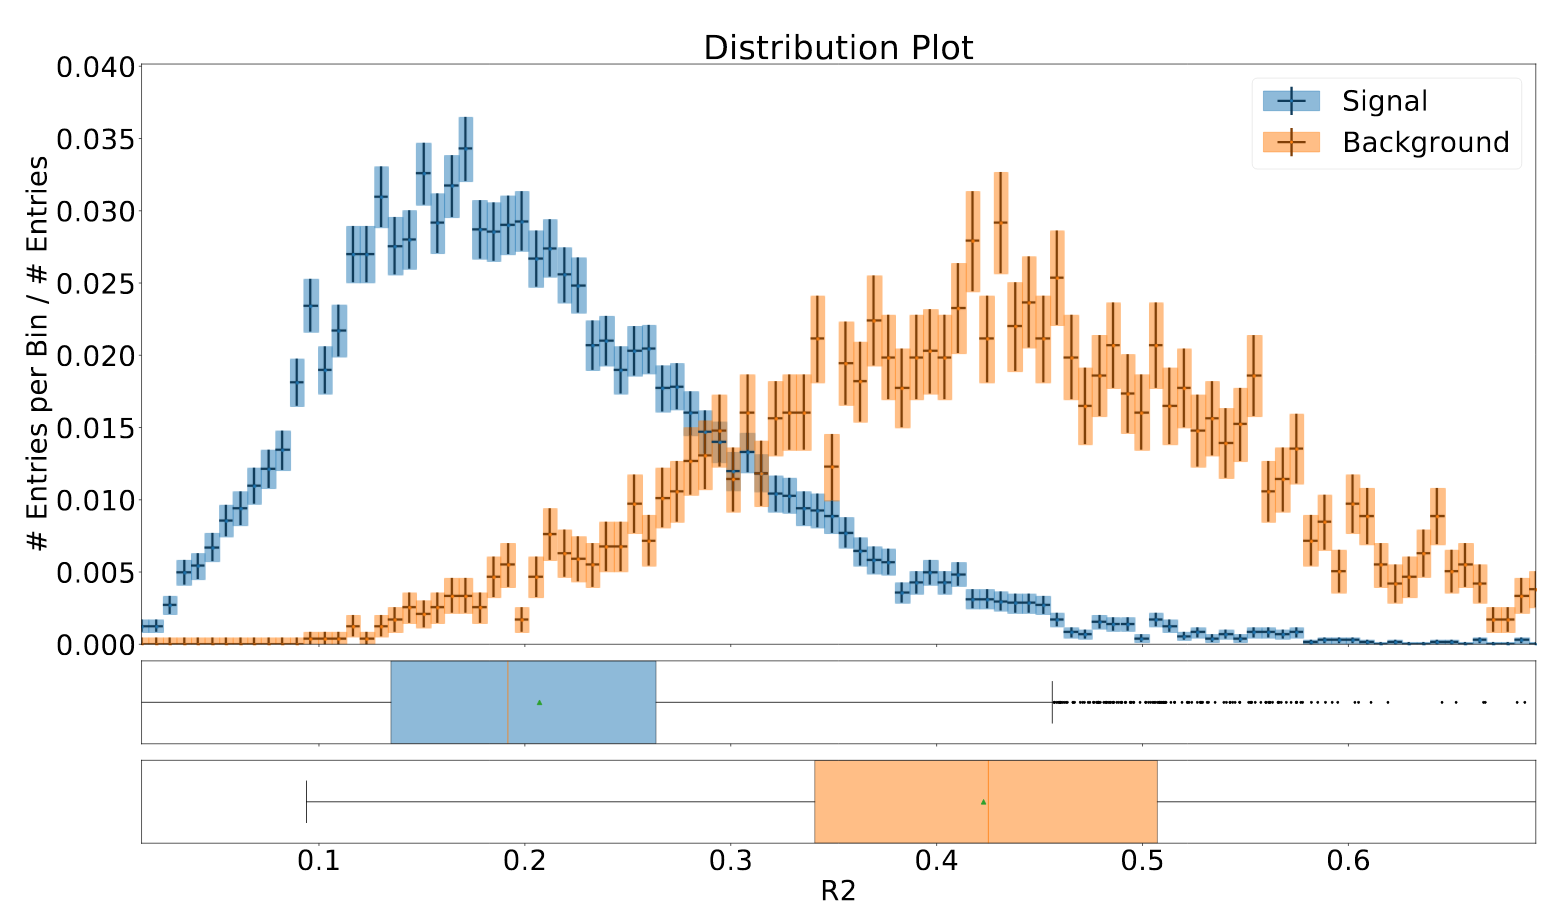
\includegraphics[width=0.7\linewidth]{r2}
	\caption{$R_2$ is the ratio of the second to the zeroth KSFW momentum in Equation \ref{eq:ksfw}. Its distribution in generic MC sample which serves as the highest weight as a variable in discriminating the continuum events, having a quite different distribution between signal and background.}
	\label{fig:R2}
\end{figure}



  In order to maximize suppression power in this analysis, these variables (KSFW, CLEO cone momentum and angular distributions) are combined as an input for FastBDT classifier. The targeted variable is the continuum event truth. The MC samples using signal $B\bar{B}$ events from signal MC and continuum events from generic MC ($q\bar{q}$ component) are prepared in a ratio of their cross-section at $\Upsilon{(4S)}$ energy. The same events reconstruction procedures for $B^0$ is applied for both MC samples. Events passing the reconstruction for $B^0$ are used for training the continuum suppression classifier. The fraction of signal and background is set to 1:1 during the training.  The output of continuum suppression classifier is renamed as ``FBDT\_CS". Then we determine the cut value at 0.66 based on the maximum of \textit{FOM} curve, as shown in Figure \ref{fig:cs_fom}. The variables used in training are listed in Table \ref{tab:cs_abr} with their abbreviations and the rank of important variables is in Table \ref{tab:cs_imp}.

The correlation between these training variables are shown in Figure \ref{fig:cs_cor}. The correlation among the variables are varied in signal and background. The ROC curve and the efficiency/purity with respect to the classifier output are shown in Figure \ref{fig:cs_roc}.
\begin{table}[htpb]
	\begin{minipage}[t]{0.4\linewidth}
		\centering
		\caption{Variables and the abbreviations for CS.}
		\label{tab:cs_abr}
		\begin{tabular}{c|c}
			\hline
			Observables &  Abbreviations\\
			\hline
			CleoConeCS(9,) &  CleoC1 \\
			KSFWVariables(hoo1,) & KSFWV1 \\
			CleoConeCS(7,) & CleoC2\\
			CleoConeCS(5,) & CleoC3\\
			KSFWVariables(hso22,) & KSFWV2\\
			KSFWVariables(hoo3,) & KSFWV3\\
			CleoConeCS(4,) & CleoC4 \\
			KSFWVariables(hoo4,) &  KSFWV4\\
			CleoConeCS(3,) & CleoC5 \\
			CleoConeCS(6,) & CleoC6\\
			CleoConeCS(8,) & CleoC7\\
			KSFWVariables(hso14,) &   KSFWV5\\
			KSFWVariables(hso00,) & KSFWV6\\
			KSFWVariables(et,) & KSFWV7\\
			KSFWVariables(hso24,) & KSFWV8\\
			KSFWVariables(hso04,) & KSFWV9\\
			KSFWVariables(hso20,) & KSFWV10 \\
			KSFWVariables(mm2,)  & KSFWV11\\
			KSFWVariables(hoo2,) &  KSFWV12\\
			thrustOm & thrus1 \\
			cosTBz & cosTB1\\
			CleoConeCS(1,) & CleoC8 \\
			CleoConeCS(2,) & CleoC9 \\
			KSFWVariables(hso02,) &  KSFWV13\\
			KSFWVariables(hoo0,) &  KSFWV14 \\
			KSFWVariables(hso12,) &  KSFWV15\\
			KSFWVariables(hso10,) & KSFWV16\\
			cosTBTO & cosTB2\\
			thrustBm & thrus2\\
			R2 & R2\\
			\hline
		\end{tabular}
	\end{minipage}
	\begin{minipage}[t]{0.5\linewidth}
		\centering 
		\caption{The rank of important variables for CS. }
		\label{tab:cs_imp}
		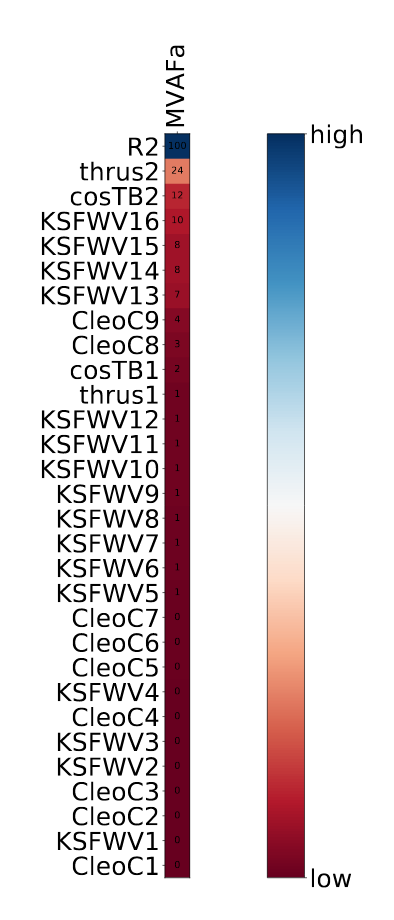
\includegraphics[width=4cm]{cs-imp}
	\end{minipage}
\end{table}

\begin{figure}[ht]
	\begin{minipage}[b]{0.5\linewidth}
		\centering 
		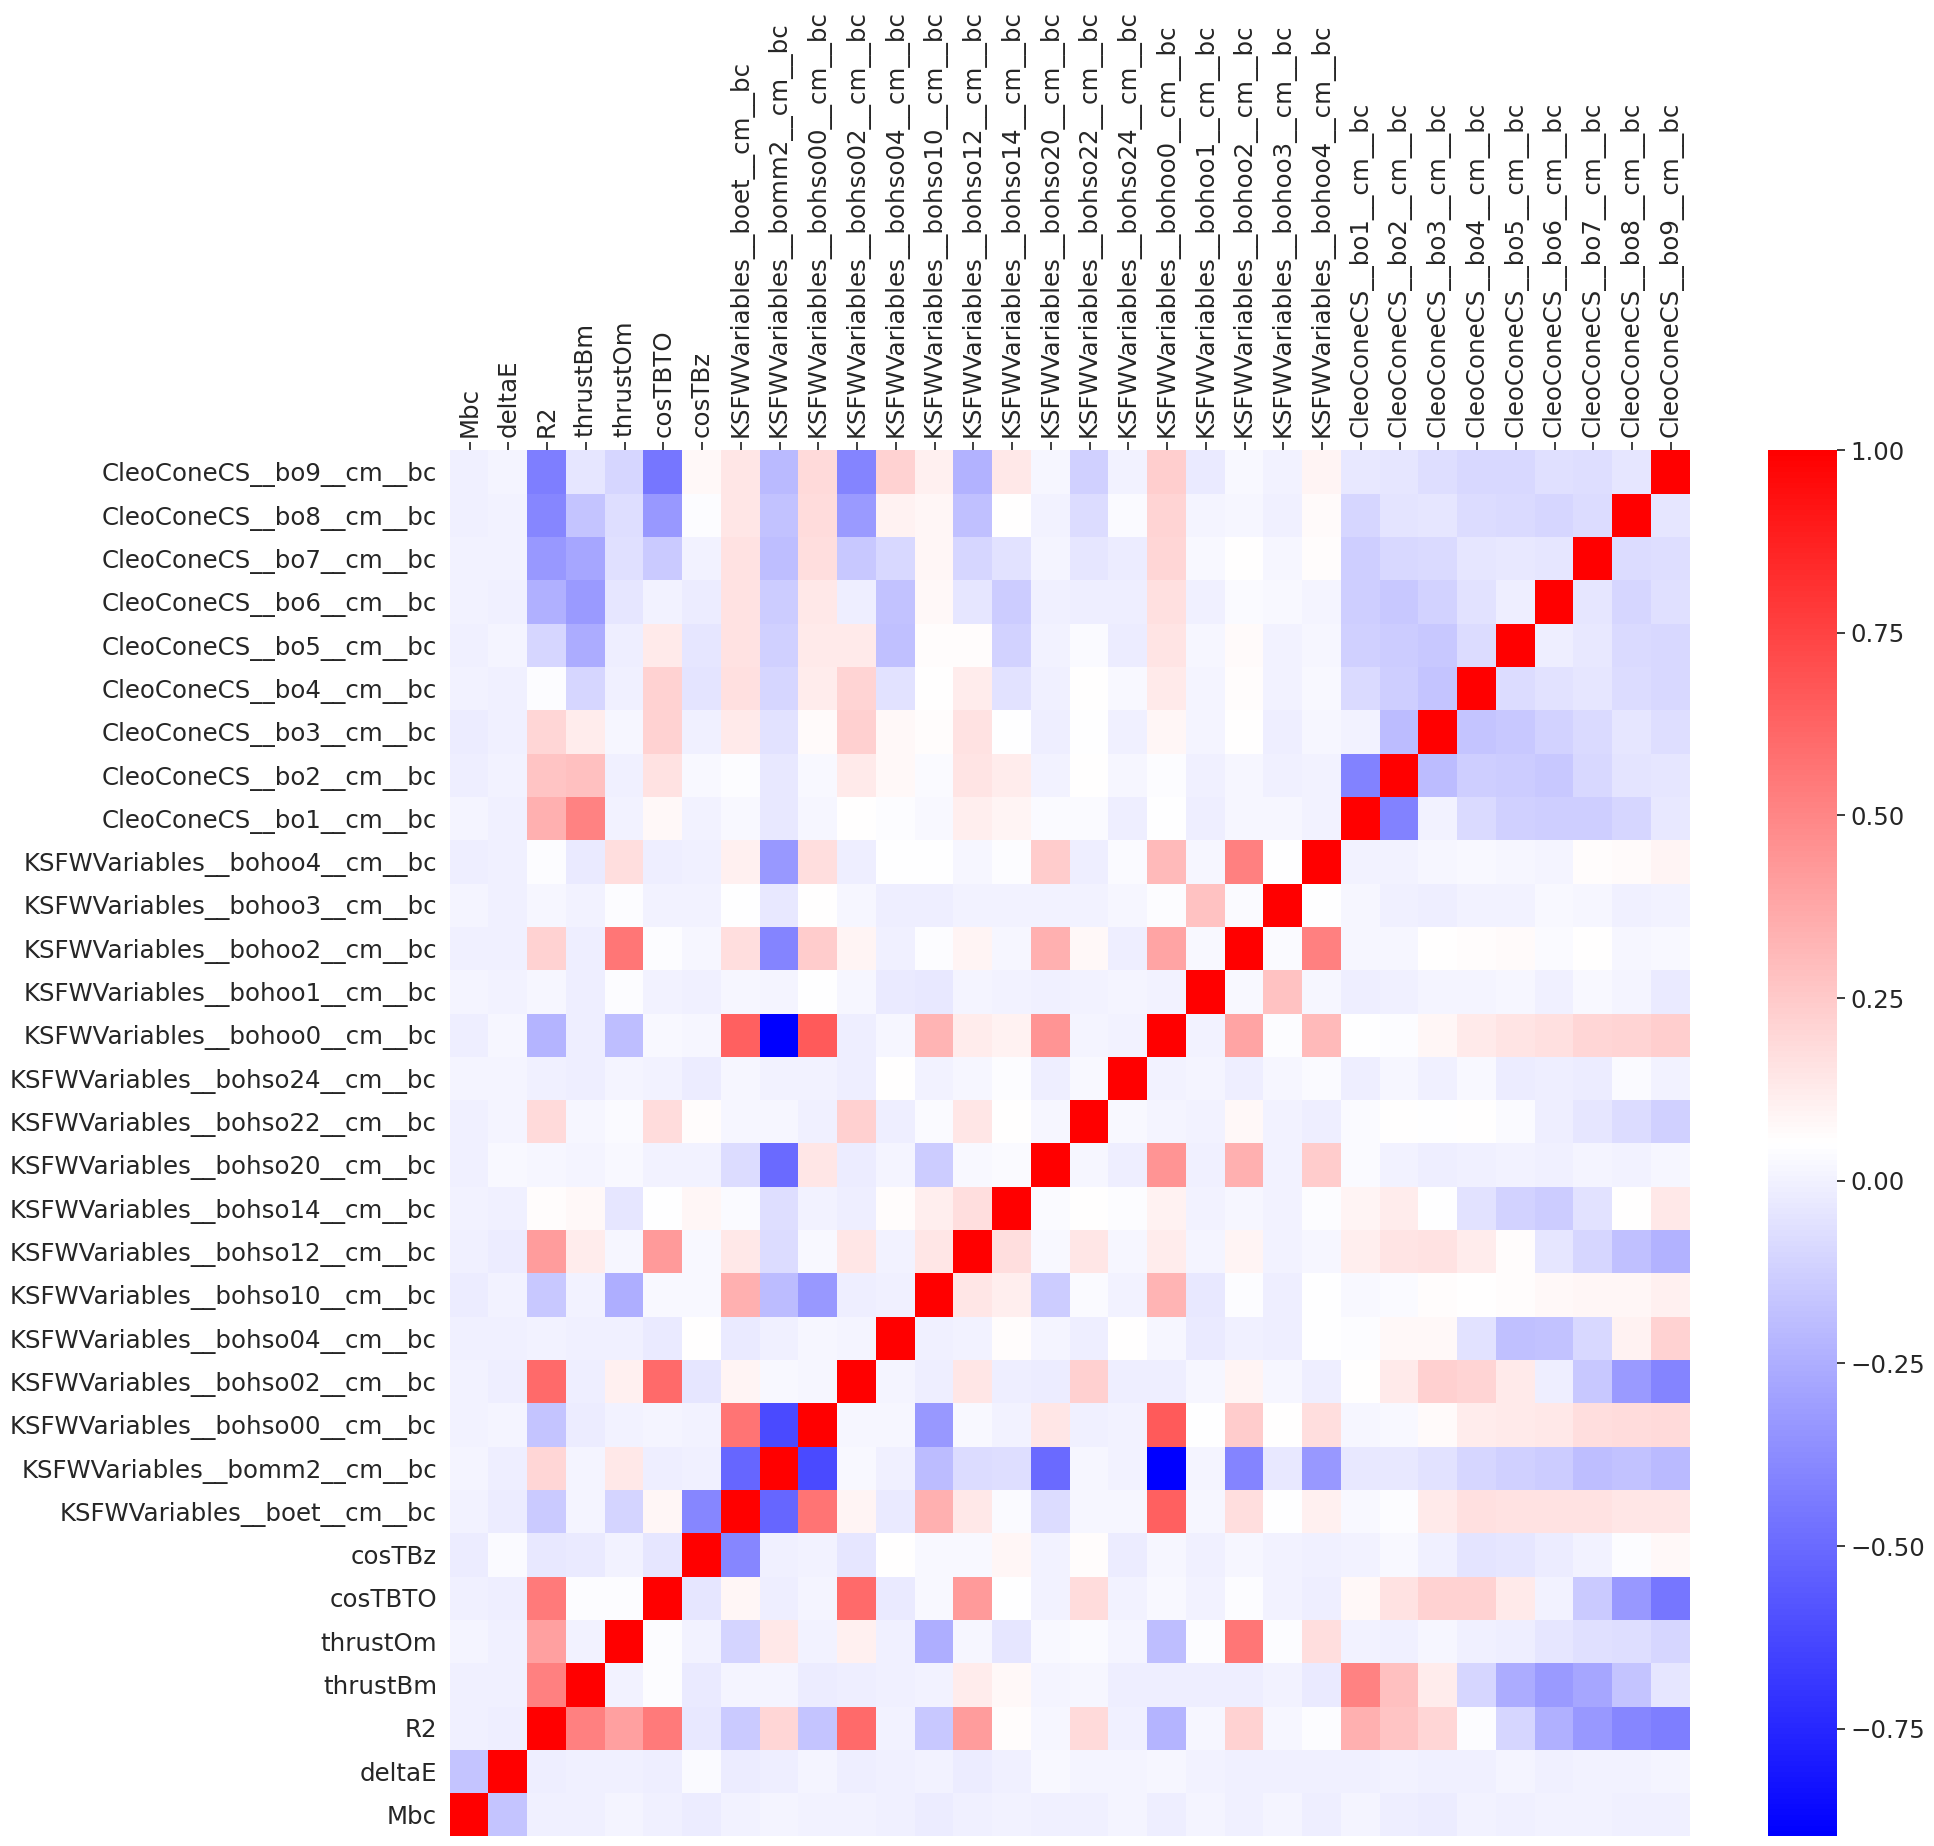
\includegraphics[height=7cm]{figures/corr_cs_kine_sig}	
	\end{minipage}
\begin{minipage}[b]{0.5\linewidth}
	\centering 
	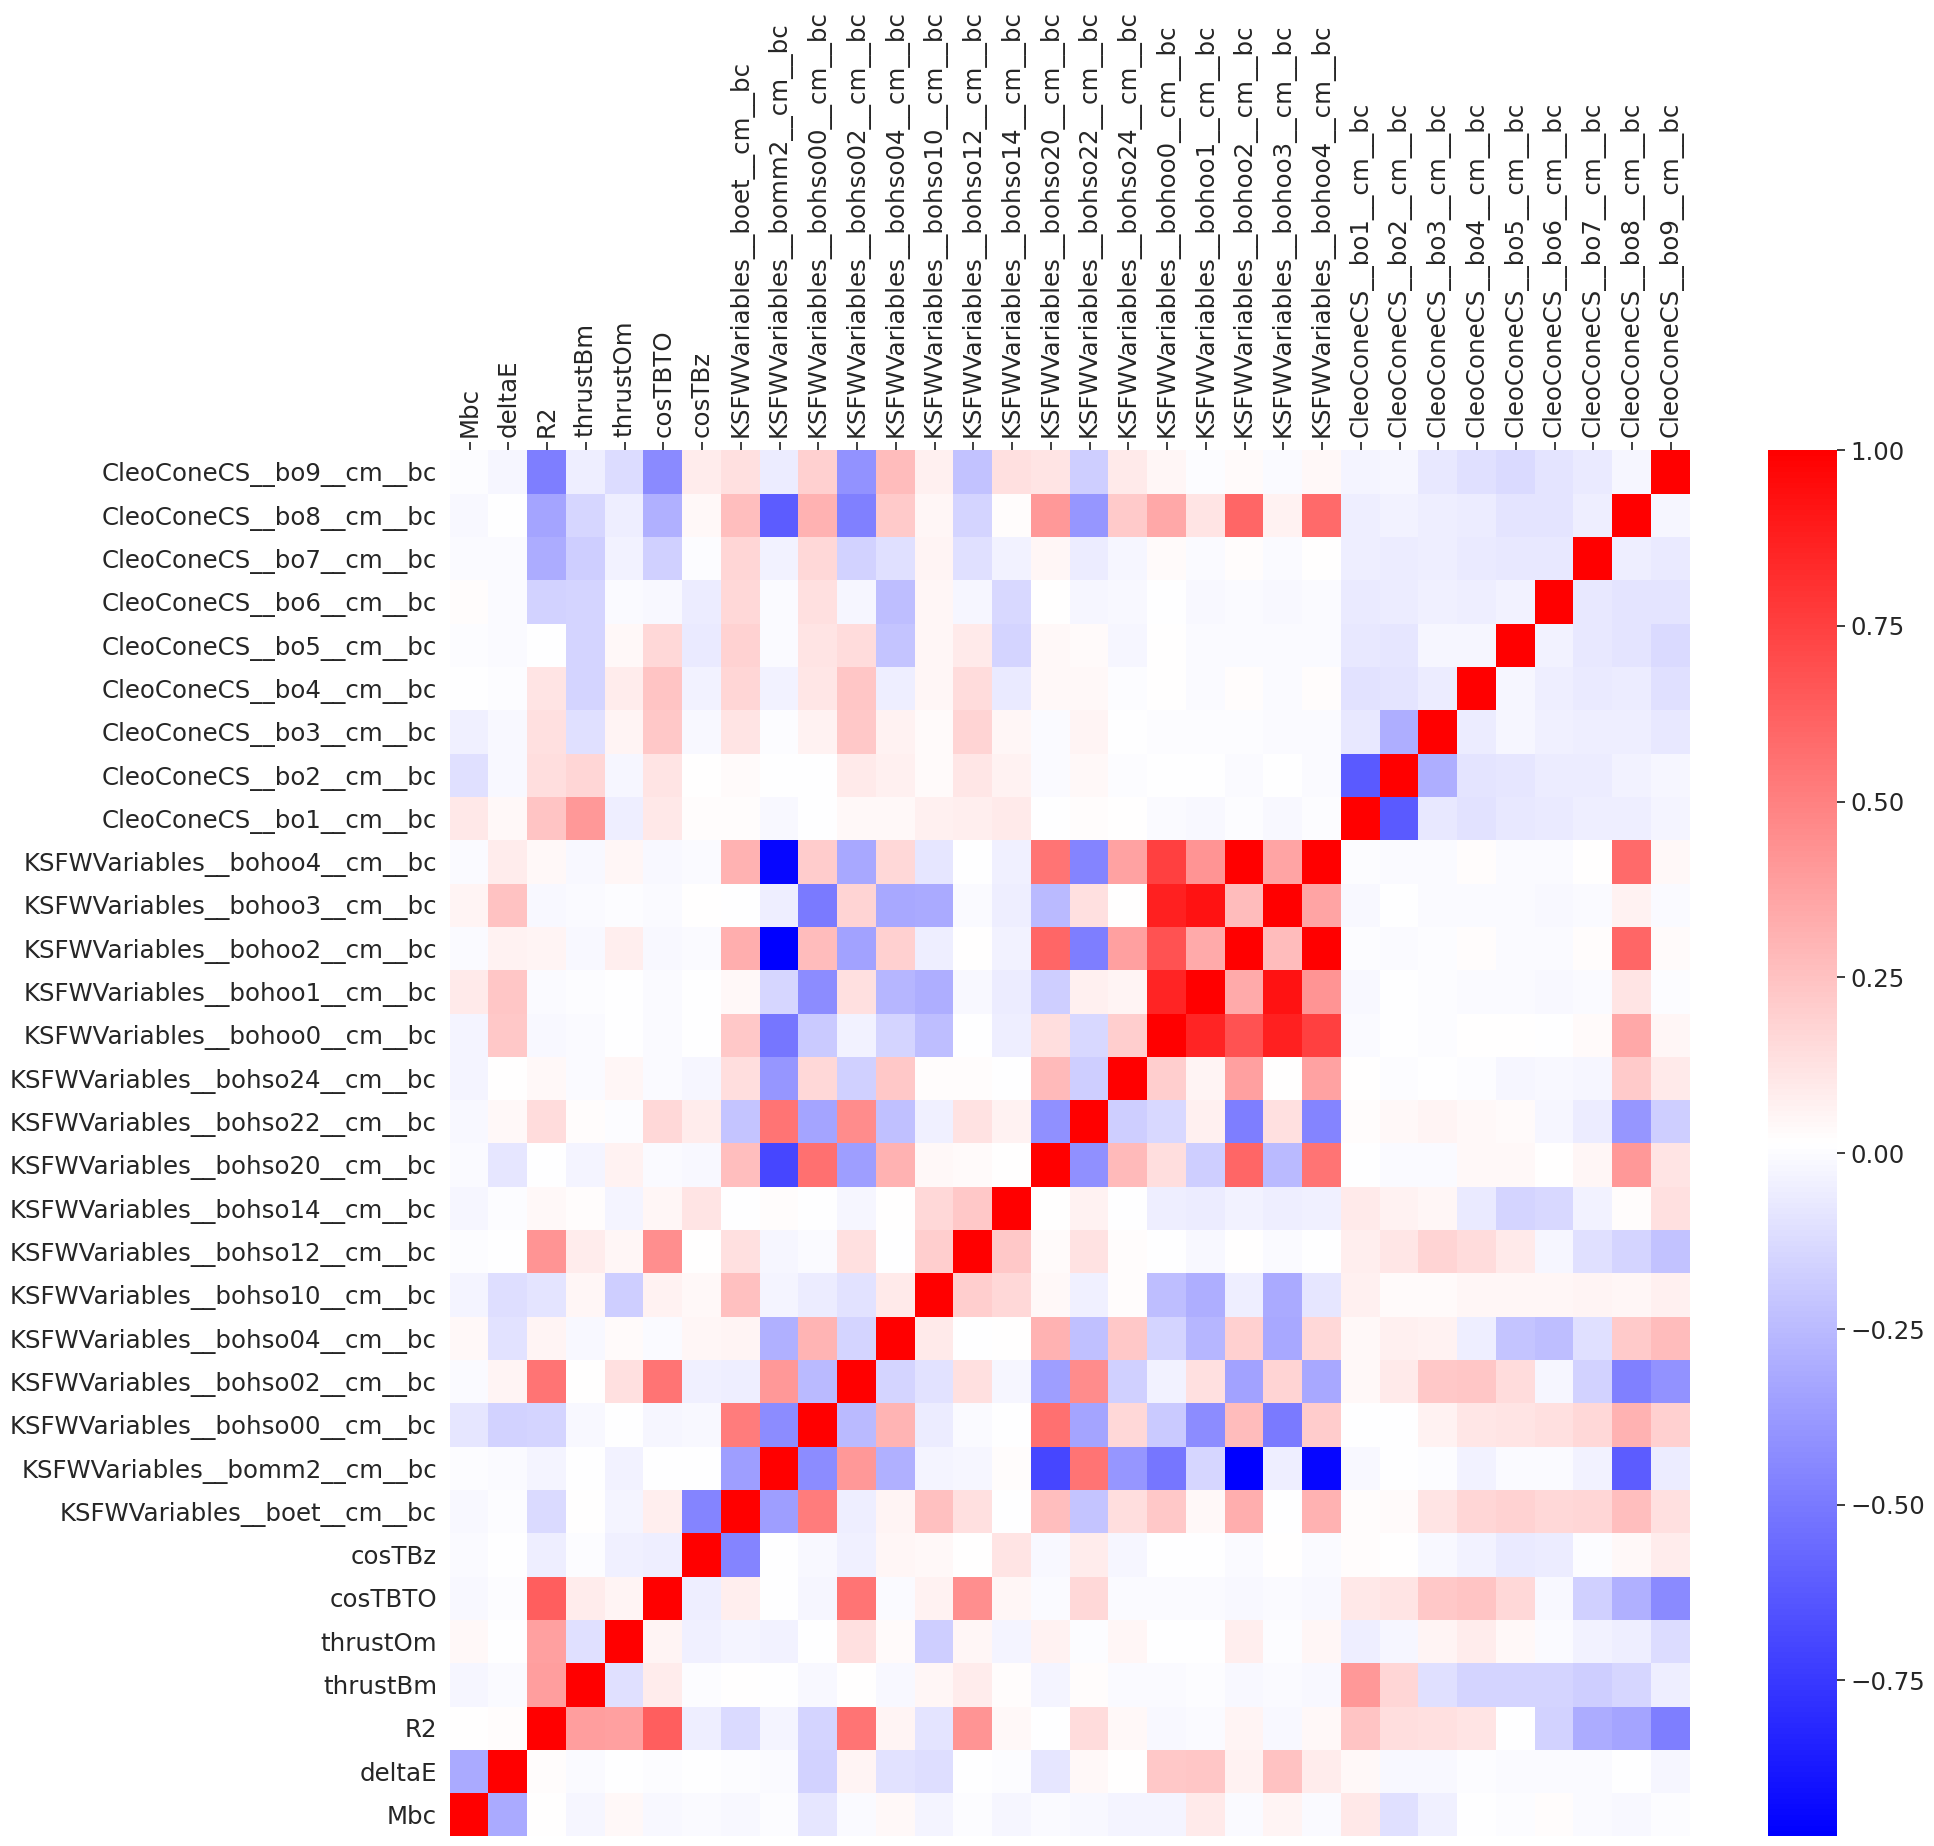
\includegraphics[height=7cm]{figures/corr_cs_kine_bkg}	
\end{minipage}
	\caption{The correlation in variables for continuum suppression. The left is for signal and the right is for background.}
	\label{fig:cs_cor}
\end{figure}

\begin{figure}[ht]
	\begin{minipage}[b]{0.5\linewidth}
		\centering 
		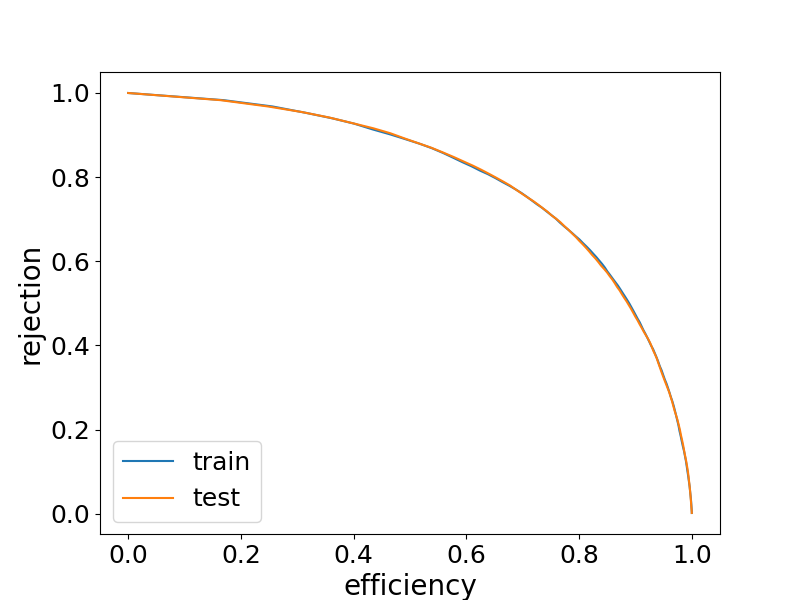
\includegraphics[height=5cm]{figures/ROC_CS}	
	\end{minipage}
	\begin{minipage}[b]{0.5\linewidth}
		\centering 
		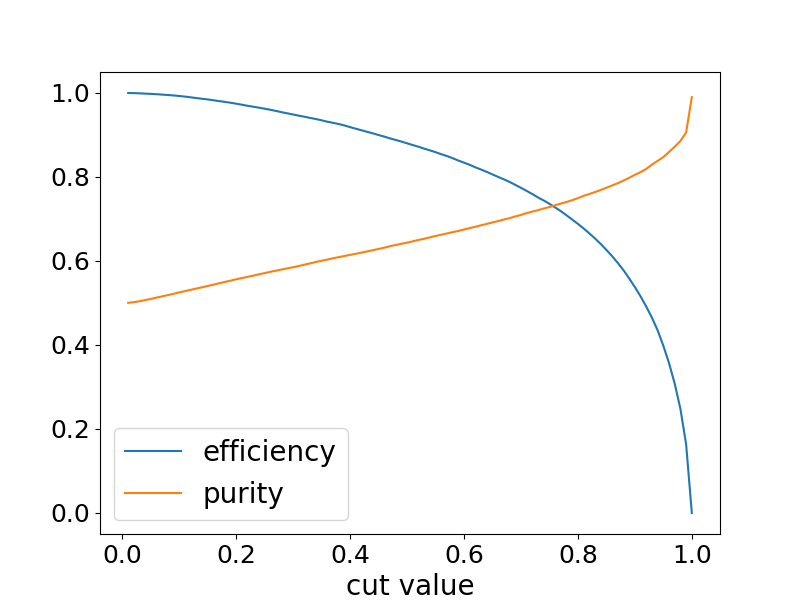
\includegraphics[height=5cm]{figures/eff_CS}	
	\end{minipage}
\caption{The left is the ROC curve (blue for training and orange for testing)
	and the right is the efficiency(blue) and purity(orange) regarding the classifier output ``FBDT\_CS"}
	\label{fig:cs_roc}
\end{figure}

Overtraining check is made by comparing the distribution of signal and background depending on the classifier output in both training and testing samples. The testing samples show about 1\% lower in each bin for both signal and background events, which is within the acceptable range.  
\begin{figure}[H]
	\centering
	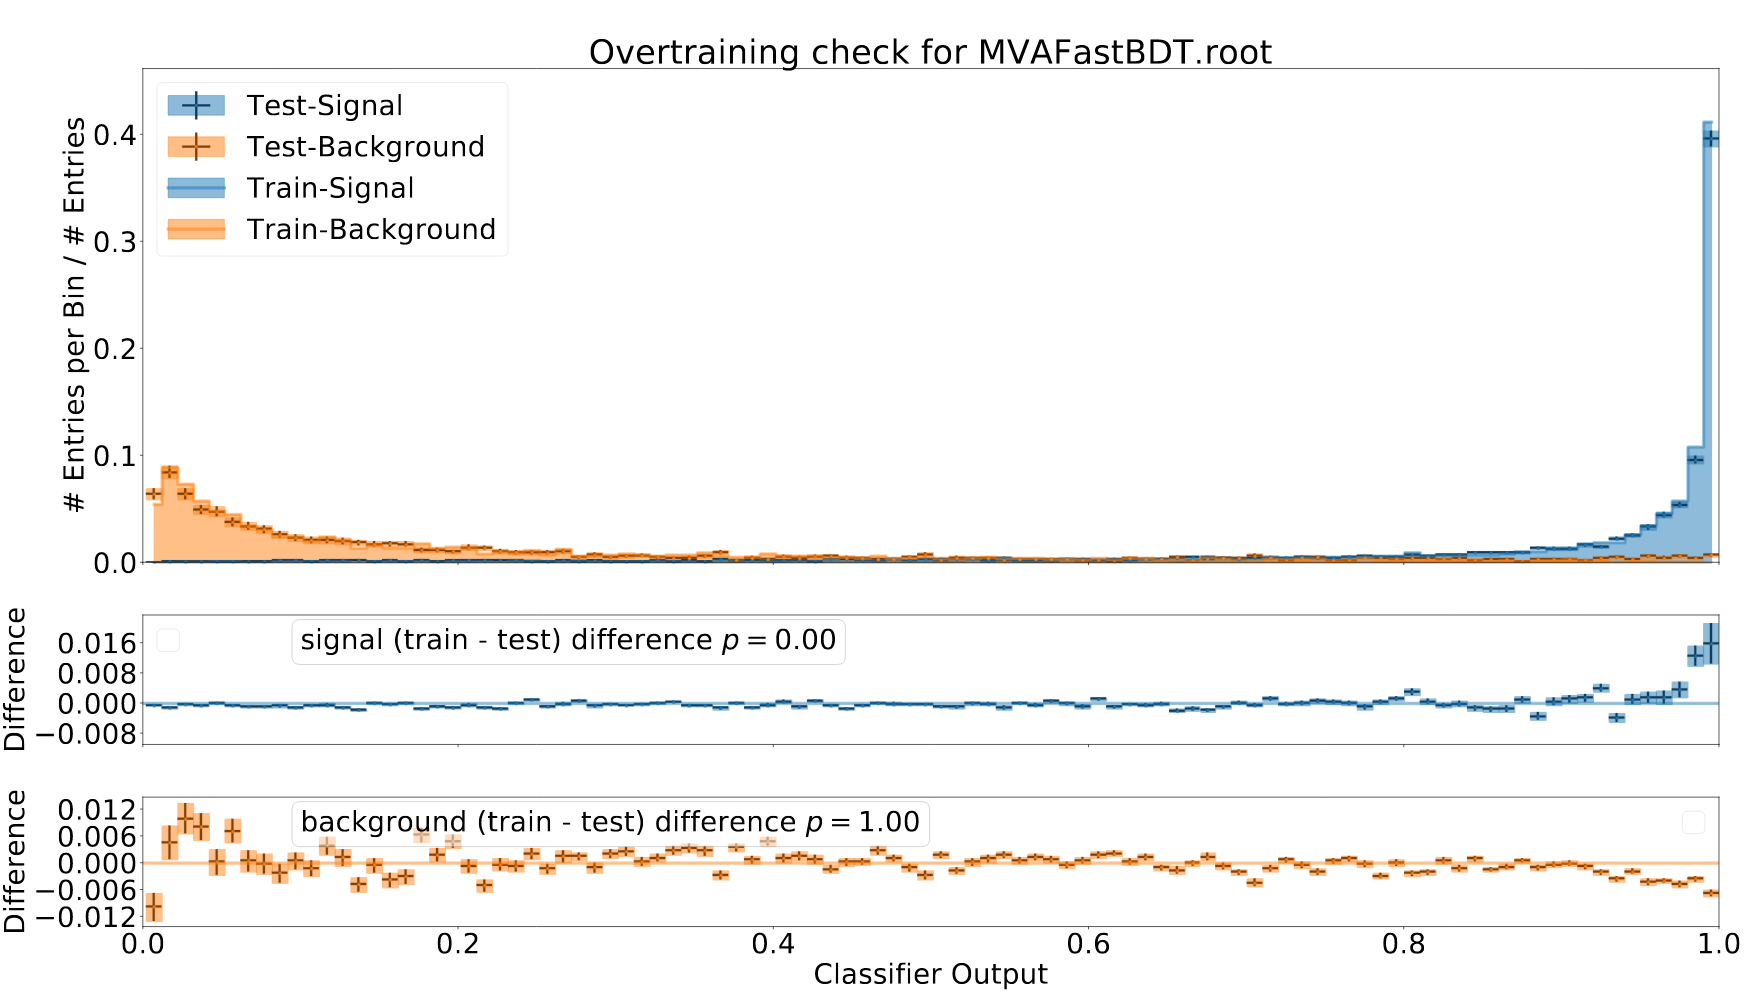
\includegraphics[width=0.8\linewidth]{cs-overtrain}
	\caption{Over-training check of continuum classifier, where a very small difference in training and testing (1\%) is shown.}
\end{figure}

\begin{figure}[H]
	\centering
	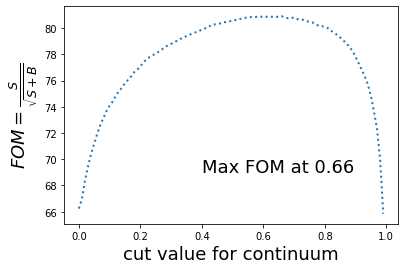
\includegraphics[width=0.6\linewidth]{cs-fom}
	\caption{\textit{FOM} depending on the cut value of continuum classifier output, cut value at 0.66 is used for continuum suppression. }
	\label{fig:cs_fom}
\end{figure}

% summary of $B^0$ stats goes here
\subsection{Resonance Background}
Besides the major contribution from continuum background, charmonium resonance that mediates through $b \to c$ transition brings odd $\textit{CP}$ eigenvalue in the final states as same as $B^0 \to K_S^0  K_S^0  K_S^0$. Monitoring their contribution is also important. Basically, one needs to check the resonance states formed by two $K_S^0$ with corresponding invariant mass. In $B^0 \to X(K_S^0 K_S^0) K_S^0$,  there are two types of resonant events that give out same final states, one is resonant signal and the other is resonant background. For $b \to s$ transitions as resonance signal because of the $\it{CP}$-even final states, \textit{X} could be $f_2(1270)$, $f_0(1500)$, $f_{2}^{'}(1525)$, $f_0(980)$, $f_0(1710)$ and $f_2(2010)$. For $b \to c$ transition as resonance background because of $\it{CP}$-odd final states, \textit{X} could be $D^0$, $J/\psi$, $\psi(2S)$,  $\chi_{c0}$, $\chi_{c1}$, and $\chi_{c2}$.

The number of these background in signal reconstruction could be further reduced by implementing veto on invariant mass of 2$K_S^0$. However, such veto should be carefully validated with data. The distribution of invariant mass of \textit{X} should agree well in MC and data, which is hard to check in the low luminosity. The distribution of 2$K_S^0$ invariant mass in generic MC and data are shown in the Appendix 


 Some of these resonance have not been implemented inside generic MC production in the current Belle II simulation. Given the very limited statistics of data accumulation we used in this analysis, we only present the expected number of these resonances in 400$fb^{-1}$ luminosity (about $2.14 \times 10^8$ events) from generic $\Upsilon{(4S)}$ events. These numbers should be re-checked in the future when data accumulation increases, and veto must be based on the structure of 2$K_S^0$ invariant mass from data as well. Details about the expected yields can be found in Table \ref{tab:f_res}. Currently there is no veto applied for rejecting these resonant background considering the estimated background number is about 1 event in the current luminosity.
\begin{sidewaystable}
	\caption{Expected yield for signal and background resonances $2.14\times 10^8 B\bar{B}$ in generic MC. The branching fraction of $B\to X K_S$ and $X \to 2K_S$ are listed for both PDG value and value in Belle II DEC. file. The number expected from $\it{CP}$-odd contamination is very low at current luminosity.  }
	\label{tab:f_res}
	\centering
	\begin{tabular}{|c|c|c|c|c|c|c|}
		\hline
		Resonances & Br($B \to X K_S$)PDG  & Br($X \to2K_S$) & Br($B \to X K_S$)Dec. & Br($X \to2K_S$)Dec. & $B\bar{B}$ pairs & Expected yields \\
		\hline
		$D^0 K_S$ & $2.6 \times 10^{-5}$ & $1.7\times 10^{-4}$ & $2.6 \times 10^{-5}$ & $1.8\times 10^{-4}$ & $2.14\times 10^8$ & 0.134 \\
		\hline
		$\eta K_S$ & $3.45\times 10^{-4}$ & $<3.1\times 10^{-4}$ & $4\times 10^{-4}$ & No Value & $2.14\times 10^8$ & No Value  \\
		\hline
		$J/\psi K_S$ & $4.35\times 10^{-4}$ & $<1.4\times 10^{-8}$ & $4.35\times 10^{-4}$ & 0 & $2.14\times 10^8$ & 0 \\
		\hline
		$\psi(2S)K_S$ & $2.9\times 10^{-4}$ & $<4.6\times 10^{-6}$ & $2.9\times 10^{-4}$ & 0 & $2.14\times 10^8$ & 0 \\
		\hline
		$\chi_{c0}K_S$ & $7.3\times 10^{-5}$ & $3.16\times 10^{-3}$ & $7.35\times 10^{-5}$ & $3.1\times 10^{-3}$ & $2.14\times 10^8$ & 6.21 \\
		\hline
		$\chi_{c1}K_S$ & $1.96\times 10^{-4}$ & $6\times 10^{-5}$ & $1.96\times 10^{-4}$ & $1\times 10^{-5}$ & $2.14\times 10^8$ & 0.05 \\
		\hline
		$\chi_{c2}K_S$ & $7.5\times 10^{-6}$ & $2.6\times 10^{-4}$ & $7.5\times 10^{-6}$ & $5.5\times 10^{}-4$ & $2.14\times 10^8$ & 0.11 \\
		\hline
		$f_2(1270)K_S$ & $1.35\times 10^{-6}$ & $1.15\times 10^{-2}$ & $1.35\times 10^{-6}$ & $1.15\times 10^{-2}$ & $2.14\times 10^8$ & 0.42 \\
		\hline
		$f_{2}^{'}(1525)K_S$ & $1.5\times 10^{-7} $ & $2.22\times 10^{-2}$ & No value & 0.22 & $2.14\times 10^8$ & No Value \\
		\hline
		$f_2(2010)K_S$ & $5\times 10^{-7}$ & No Value  & No Value  & No Value  & $2.14\times 10^8$ & No Value \\
		\hline
		$f_0(980)K_S$ & $2.7\times 10^{-6}$ & No Value & $2.75\times 10^{-6}$ & No Value & $2.14\times 10^8$ & 43.3 \\
		\hline
		$f_0(1710)K_S$ & $5\times 10^{-7}$ & No Value  & No Value  & No Value  & $2.14\times 10^8$ & No Value \\
		\hline
		$f_0(1500)K_S$ & $6.5\times 10^{-5}$ & 0.022 & No Value & 0.022 & $2.14\times 10^8$ & No Value \\
		\hline
		Total  & - & - & - & - & - & $\simeq$50 \\
		\hline
	\end{tabular}
\end{sidewaystable}


% 2021.02.10 mid
\subsection{$B\bar{B}$ background and self-cross feed}
Another possible contribution of backgrounds are the background from $B\bar{B}$ events including the charged and the neutral ones. The estimated contributions of these types can be checked with charged $B\bar{B}$ samples and the mixed samples. For this channel, the number of events from  \textbf{$B\bar{B}$} is very limited. Self-cross feed backgrounds stands for the events from the signal-like events but the tag-side particles help form a fake signal. The combined contributions from $B\bar{B}$ background and self-cross feed is about 3\% in the channel and we don't perform special treatment on them at current luminosity.

\subsection{Signal Extraction}
After determining the contribution of all kinds of background, the event selections defined in Table 4.3 is applied to signal MC, generic MC and also the data. The integral luminosity from generic MC is 1ab$^{-1}$ and the data used in this analysis is the full data set from 2019 and 2020 spring and summer. 
The official processing of data used is proc11 and bucket 9,10,11,13,14,15 and the integral luminosity is about 62.8fb$^{-1}$. To be noticed, the good runs from data has slightly lower luminosity. 

The unbinned maximum likelihood fit using RooFit package is performed to extract the signal. 2D fit using both $M_{bc}$ and $\Delta{E}$ are done by taking the probability density function as follows: 
\begin{equation}
\mathcal{P}(M_{bc},\Delta{E}) = 
f_{signal}\times \mathcal{P}_{sig}^{M_{bc}}\times\mathcal{P}_{sig}^{\Delta{E}}
+ 
(1-f_{signal})\mathcal{P}_{bkg}^{M_{bc}}\times\mathcal{P}_{bkg}^{\Delta{E}}
\end{equation}
where $\mathcal{P}_{sig}^{M_{bc}}$ and $\mathcal{P}_{sig}^{\Delta{E}}$ are Gaussian and three Gaussians function. $f_{signal}$ is fraction of signal events. $\mathcal{P}_{bkg}^{M_{bc}}$ is  primarily continuum events, and presented as Argus distribution like Eq(4.12) shows, with a preset mass threshold at $c = 5.29$ GeV. 
\begin{equation}
f(x;\chi,c)=\frac{\chi^3}{\sqrt{2\pi}\Psi(\chi)}\cdot
\frac{x}{c^2}\sqrt{1-\frac{x^2}{c^2}}\cdot
exp\begin{Bmatrix}
-\frac{1}{2}\chi^2(1-\frac{x^2}{c^2})
\end{Bmatrix}
\end{equation}
 $x$ is defined in $0<x<c$. $\chi$ and $c$ are parameters of the distribution, $\Psi(\chi)=\Phi(\chi)-\chi\phi(\chi)-\frac{1}{2}$ where $\Phi(\chi)$ and $\phi(\chi)$  cumulative distribution and probability density functions of the standard normal distribution, respectively. 
 $\mathcal{P}_{bkg}^{\Delta{E}}$  is modeled by first order Chebyshev polynomials. The shape parameters of signal events are determined by fitting to signal MC, and  then fixed as constants in fitting of 2D on $M_{bc}$ and $\Delta E$ for generic sample and data. Fitting results on signal MC are show in Fig 4-11. 
 
 
 \begin{figure}[H]
 	\begin{minipage}[b]{0.5\linewidth}
 		\centering 
 		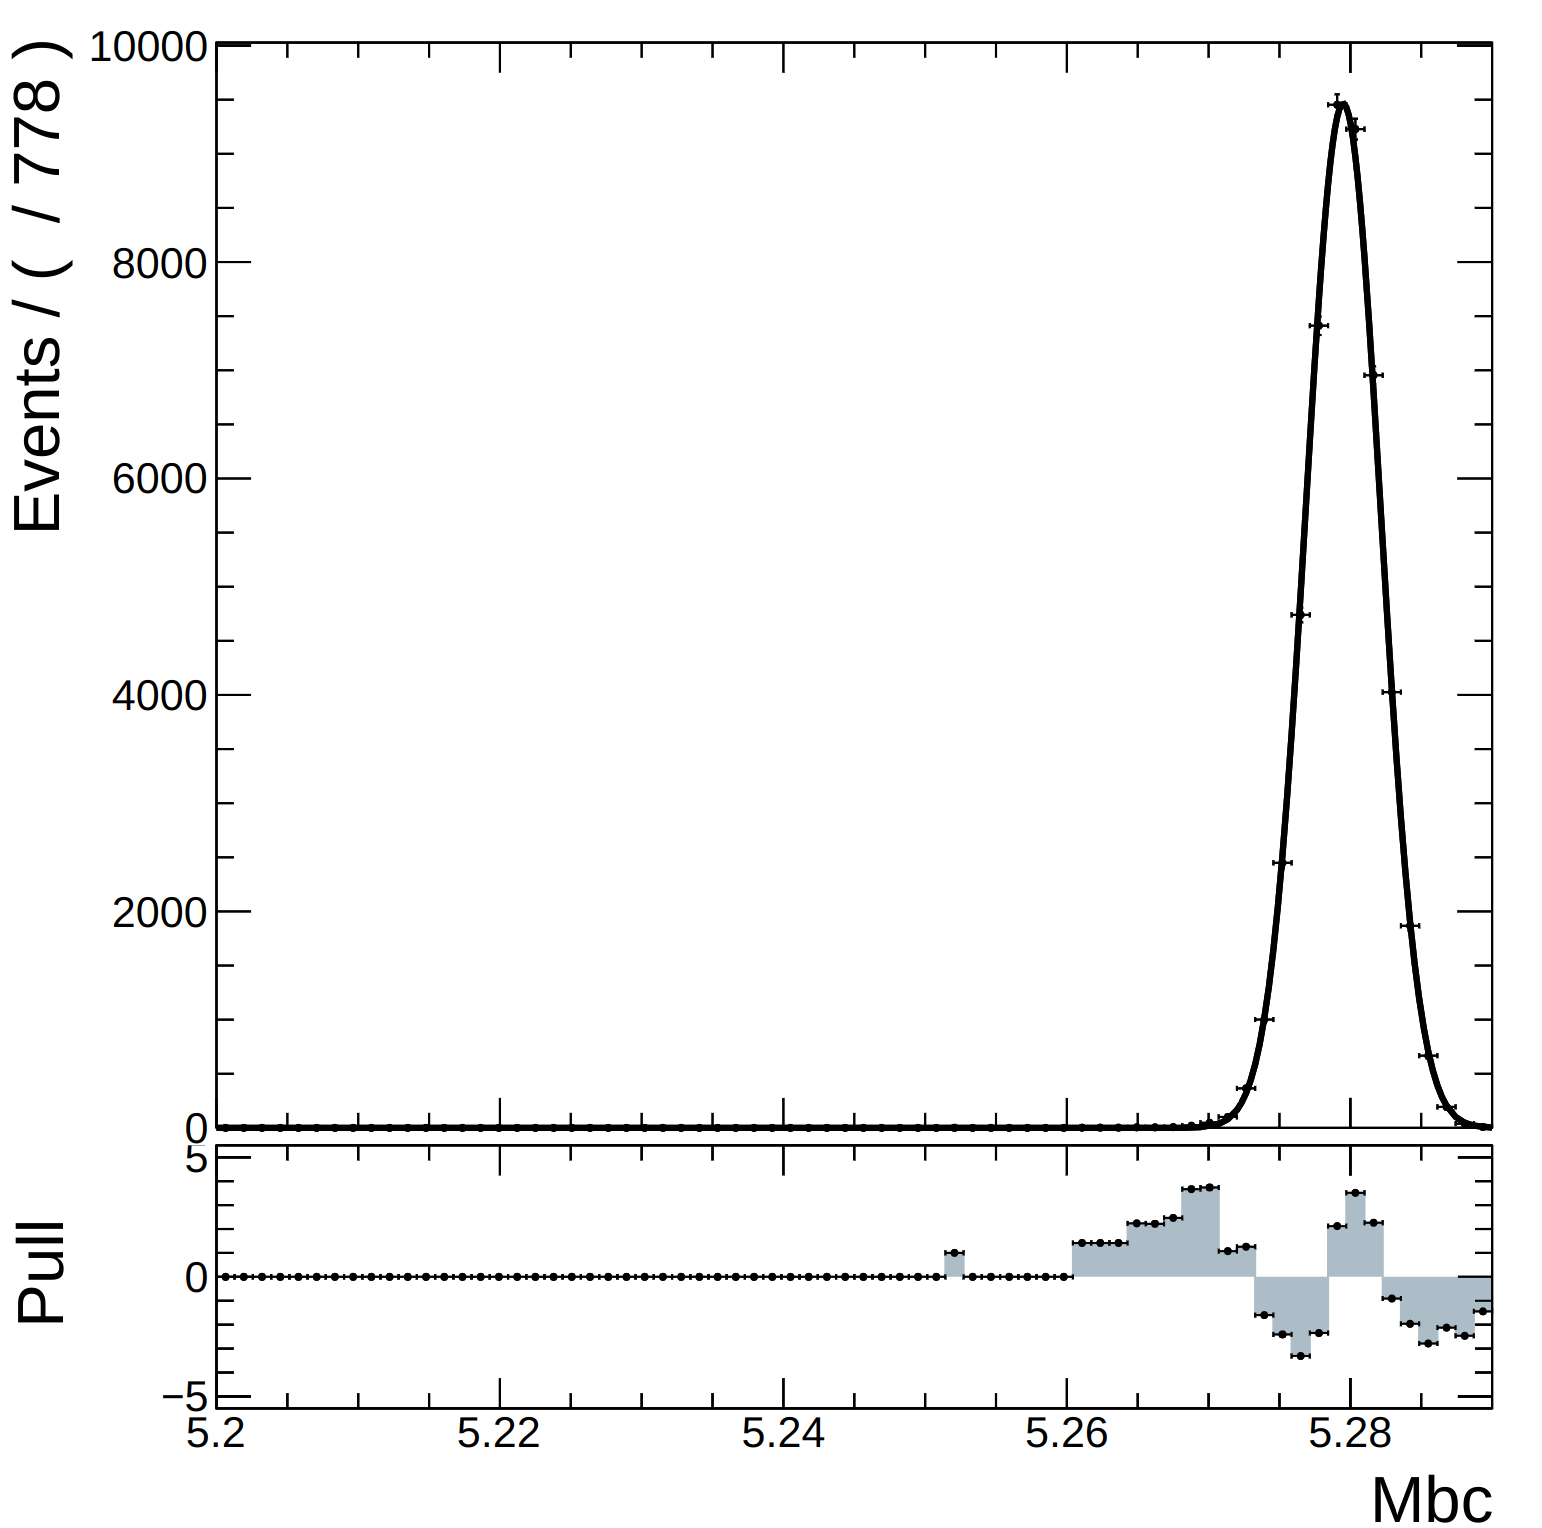
\includegraphics[height=5cm]{mbc-hist}
 		\label{fig:side:a}
 	\end{minipage}
 	\begin{minipage}[b]{0.5\linewidth}
 		\centering 
 		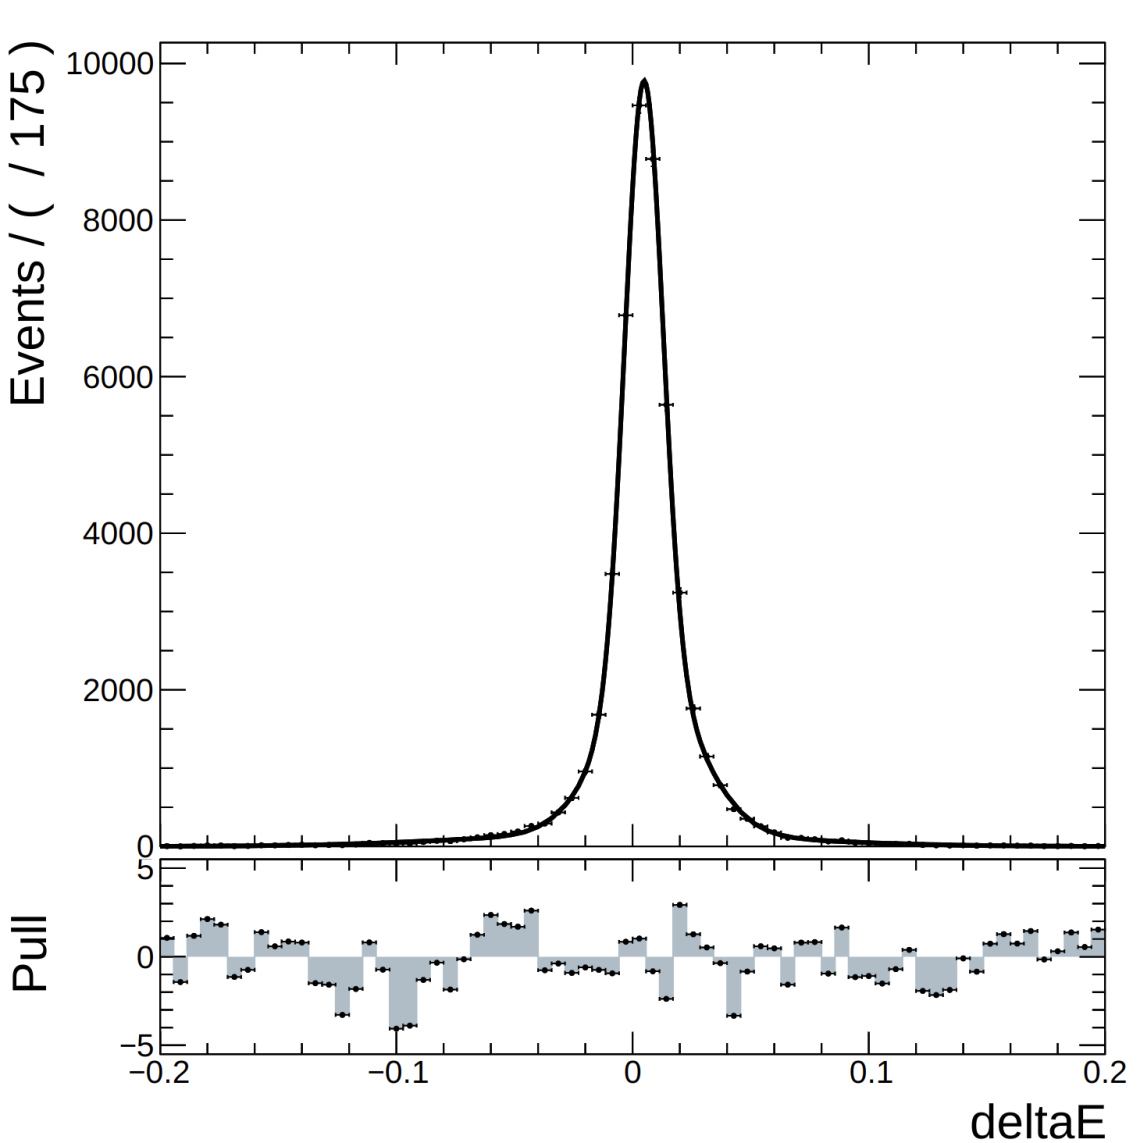
\includegraphics[height=5.2cm]{dE-hist}
 		\label{fig:side:b}
 	\end{minipage}
 	\caption{The distribution of $M_{bc}$ and $\Delta E$ of signal MC13 of $B^0 \to K_S^0  K_S^0  K_S^0$  fitted with single and triple gaussian respectively.}
 \end{figure}
\begin{comment}
\begin{table}[H]
\centering
\caption{Fit results from RooFit on $M_{bc}$ and $\Delta E$}
\begin{tabular}{|c|c|c|}
\hline
Floating Parameters  & Mean Value & +/- Error  \\
\hline
m\_mbc & 5.2795 & $4.94 \times 10^{-6}$\\
\hline
s\_mbc  & 2.6997 & $3.5\times 10^{-6}$ \\
\hline
m1\_$\Delta{E}$& $7.1063\times 10^{-3}$ & $2.63\times 10^{-5}$ \\
\hline
m2\_$\Delta{E}$& $7.8041\times 10^{-3}$ & $2.18\times 10^{-4}$ \\
\hline
s1\_$\Delta{E}$ & $1.0914\times 10^{-2}$ & $2.93\times 10^{-5}$\\
\hline
s2\_$\Delta{E}$ & $5.1961\times 10^{-2}$ & $2.02\times 10^{-5}$\\
\hline
\end{tabular}
\end{table}
\end{comment}
The continuum background is fitted also first on off-resonance generic samples to determine the shapes then fix them as constants for 2D fit, shown as follows:
\begin{figure}[H]
	\begin{minipage}[b]{0.5\linewidth}
		\centering 
		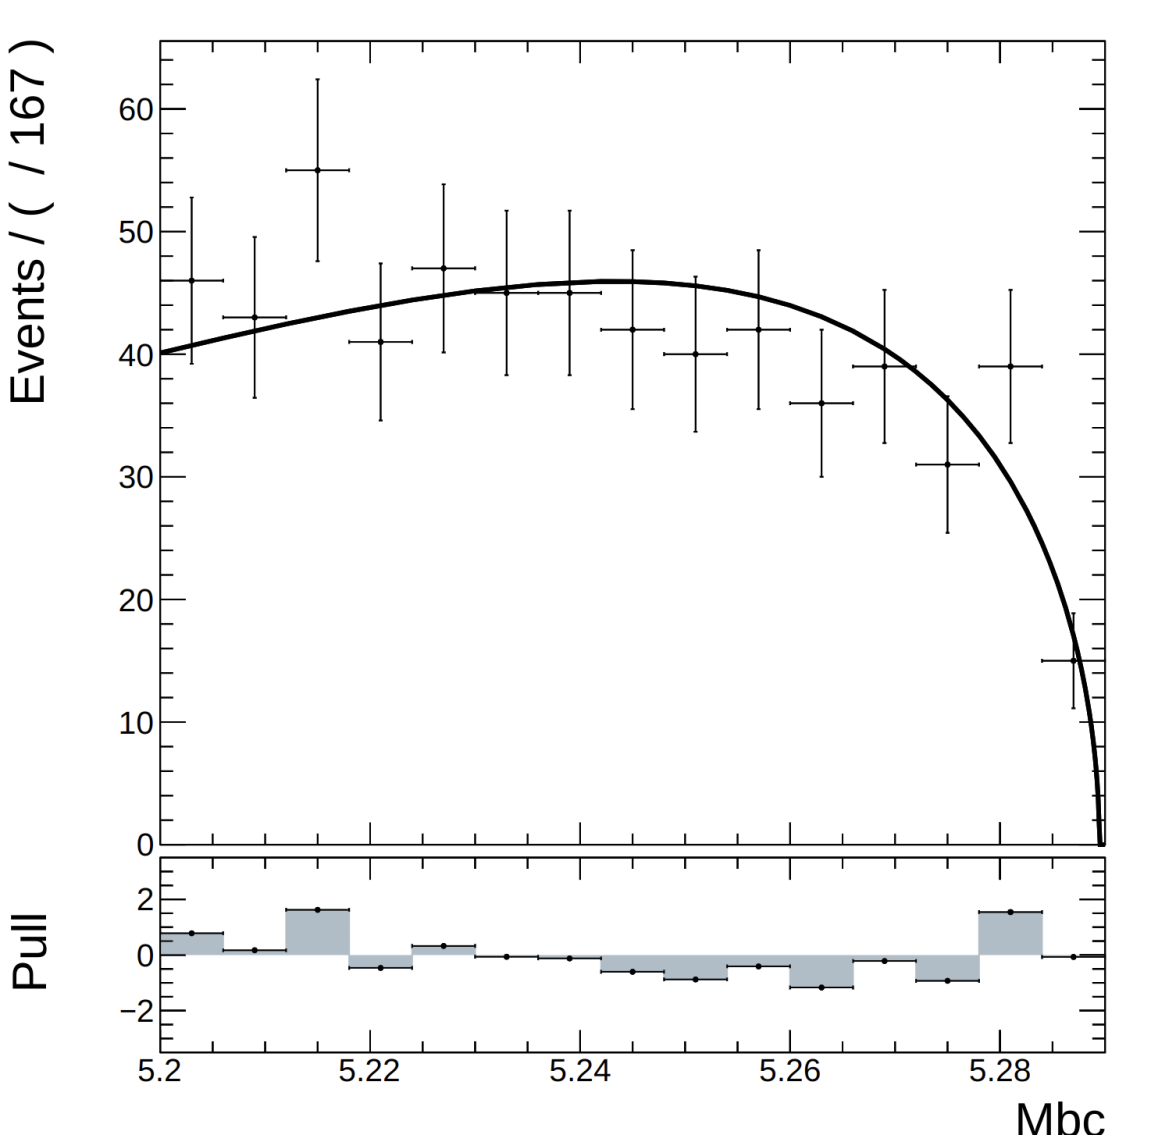
\includegraphics[height=5cm]{figures/mbc-cs-hist}
		\label{}
	\end{minipage}
	\begin{minipage}[b]{0.5\linewidth}
		\centering 
		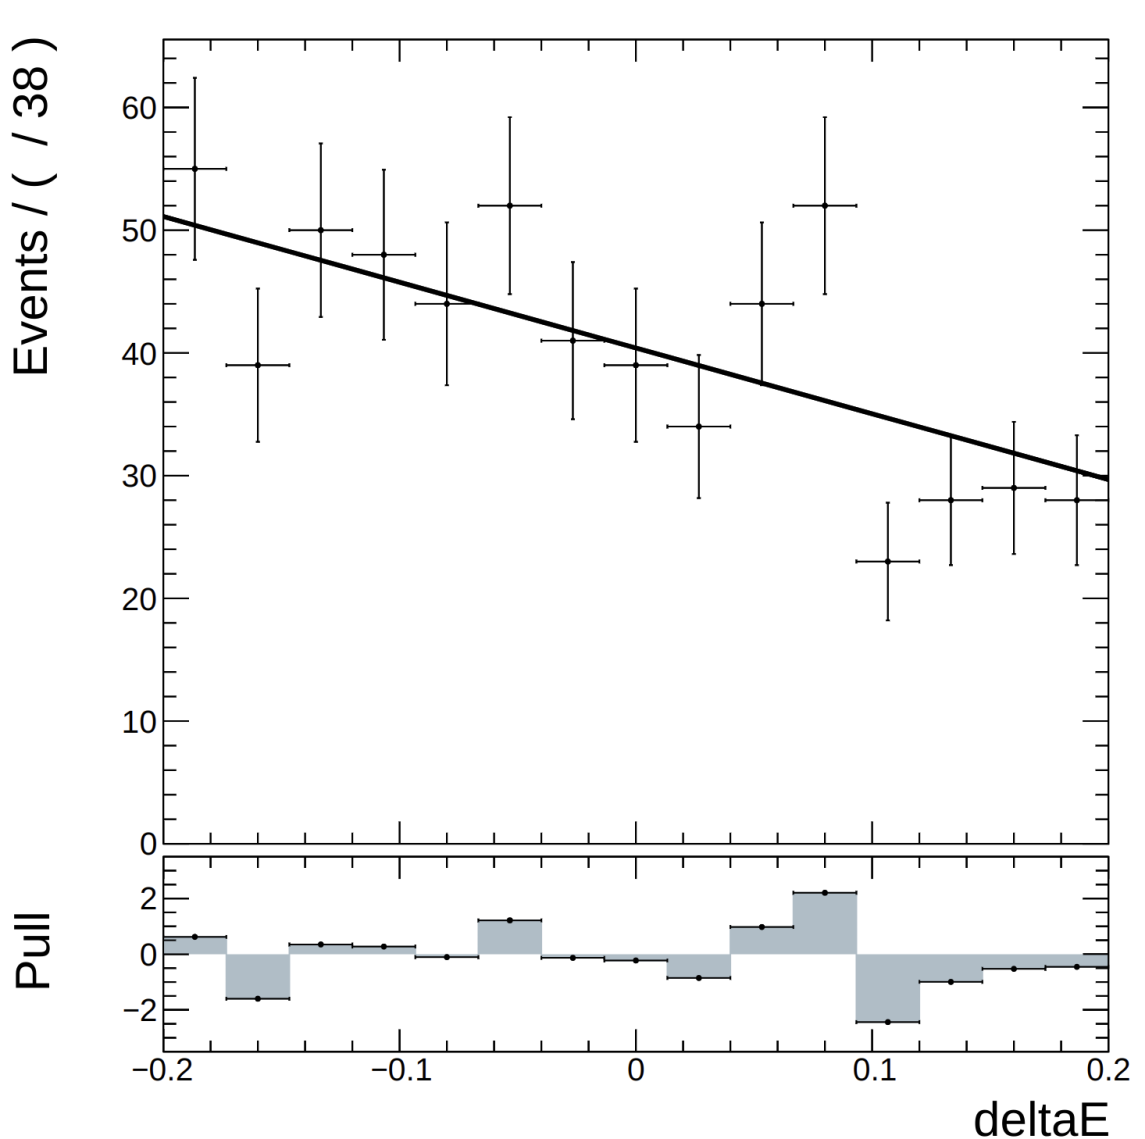
\includegraphics[height=5.2cm]{figures/dE-cs-hist}
		\label{}
	\end{minipage}
	\caption{The distribution of $M_{bc}$ and $\Delta E$ of continuum events fitted with Argus and Chebyshev polynomial respectively.}
\end{figure}

Then we set the events number for signal and background as the only parameter in float, to use Eq(4.11) 
as 2D fit functions on 1ab$^{-1}$ generic sample and data, which the fit is also done using unbinned maximum likelihood fit.
For $B^0$ in generic MC sample, the 2D fit result projected on $M_{bc}$ and $\Delta E$ is: 
\begin{figure}[H]
	\begin{minipage}[b]{0.5\linewidth}
		\centering 
		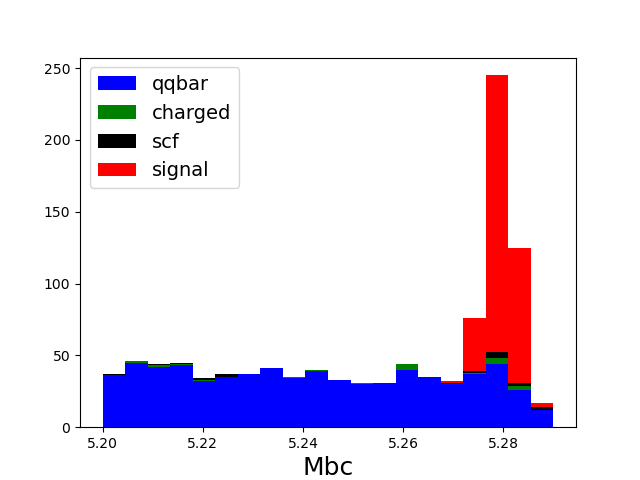
\includegraphics[height=5cm]{figures/hist_stacked_generic_mbc}
		\label{}
	\end{minipage}
	\begin{minipage}[b]{0.5\linewidth}
		\centering 
		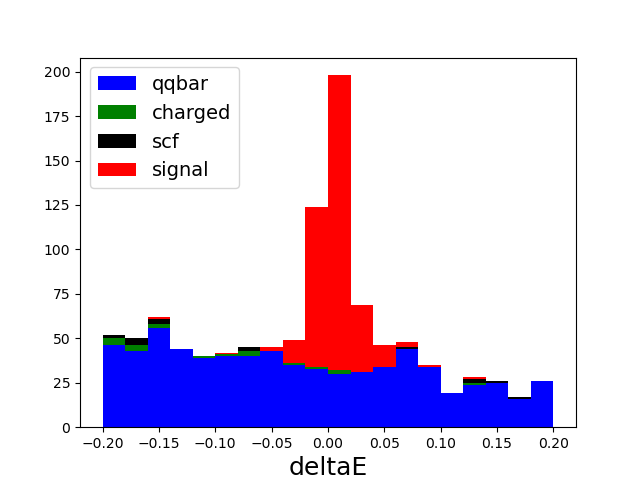
\includegraphics[height=5.2cm]{figures/hist_stacked_generic_dE}
		\label{}
	\end{minipage}
	\begin{minipage}[b]{0.5\linewidth}
		\centering 
		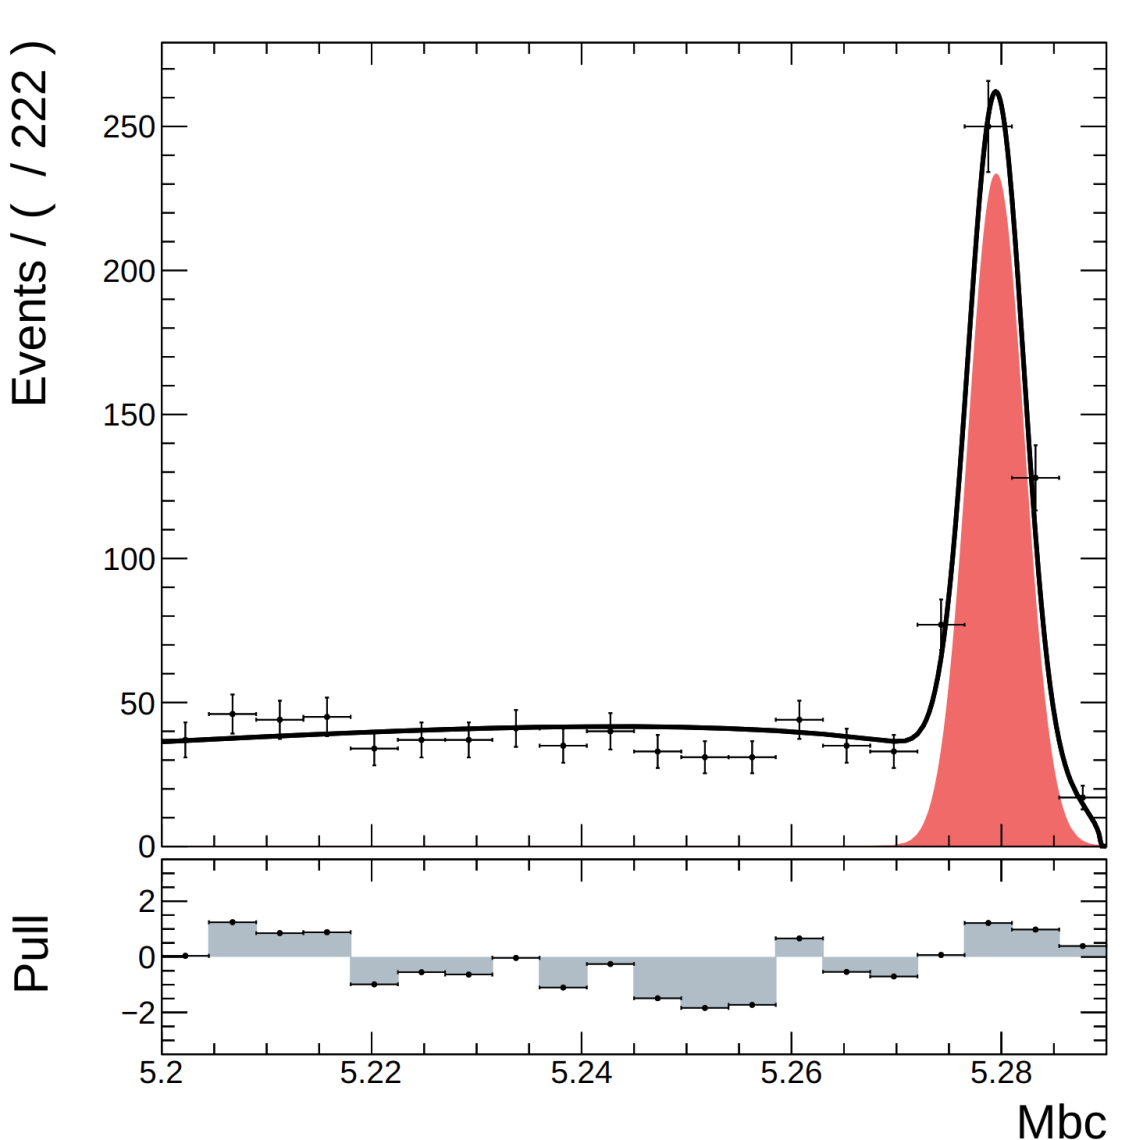
\includegraphics[height=5cm]{figures/mbc-hist-2d}
		\label{}
	\end{minipage}
	\begin{minipage}[b]{0.5\linewidth}
		\centering 
		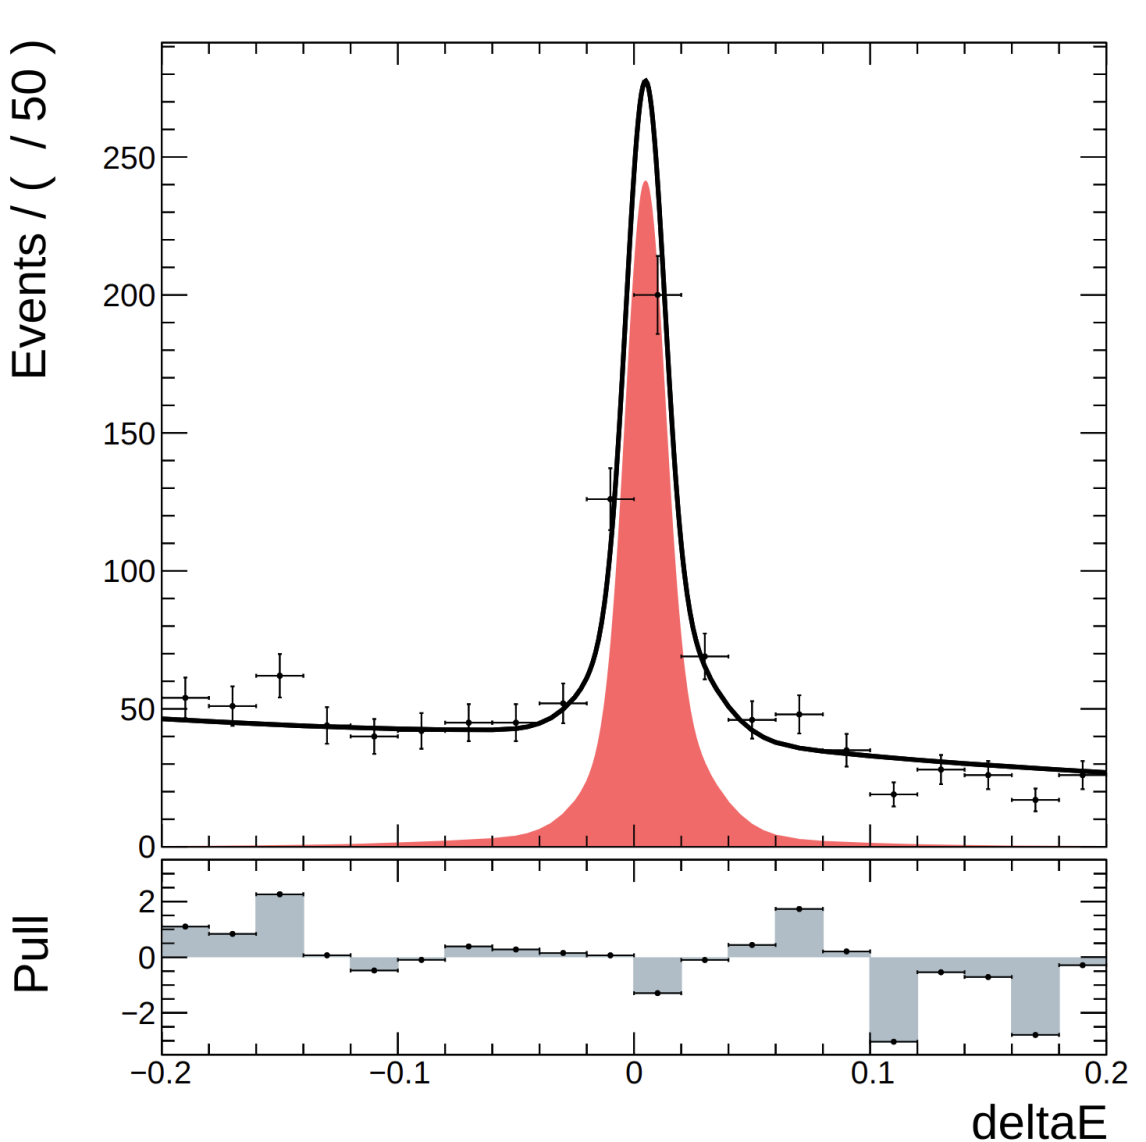
\includegraphics[height=5.2cm]{figures/dE-hist-2d}
		\label{}
	\end{minipage}
	\caption{Top is the stacked plots for generic MC of $M_{bc}$ and $\Delta E$, where each background components are stacked with signal. The bottom is the 2D fit on generic MC13, the red is signal PDF. The integral luminosity is 1 ab$^{-1}$}
\end{figure}
For the invariant mass of $K_S^0$ from $B^0$, we compared the distribution of ``InvM" and ``M" for all $K_S^0$ that have been used for $B^0$ reconstruction in data and generic MC. The distributions are shown in Fig 4-14 bottom, which the generic MC is scaled to the luminosity of data and agreed well.
For data, the 2D fit result projected on $M_{bc}$ and $\Delta E$ is in Fig 4-14 top.  
\begin{figure}[H]
	\begin{minipage}[b]{0.5\linewidth}
		\centering 
		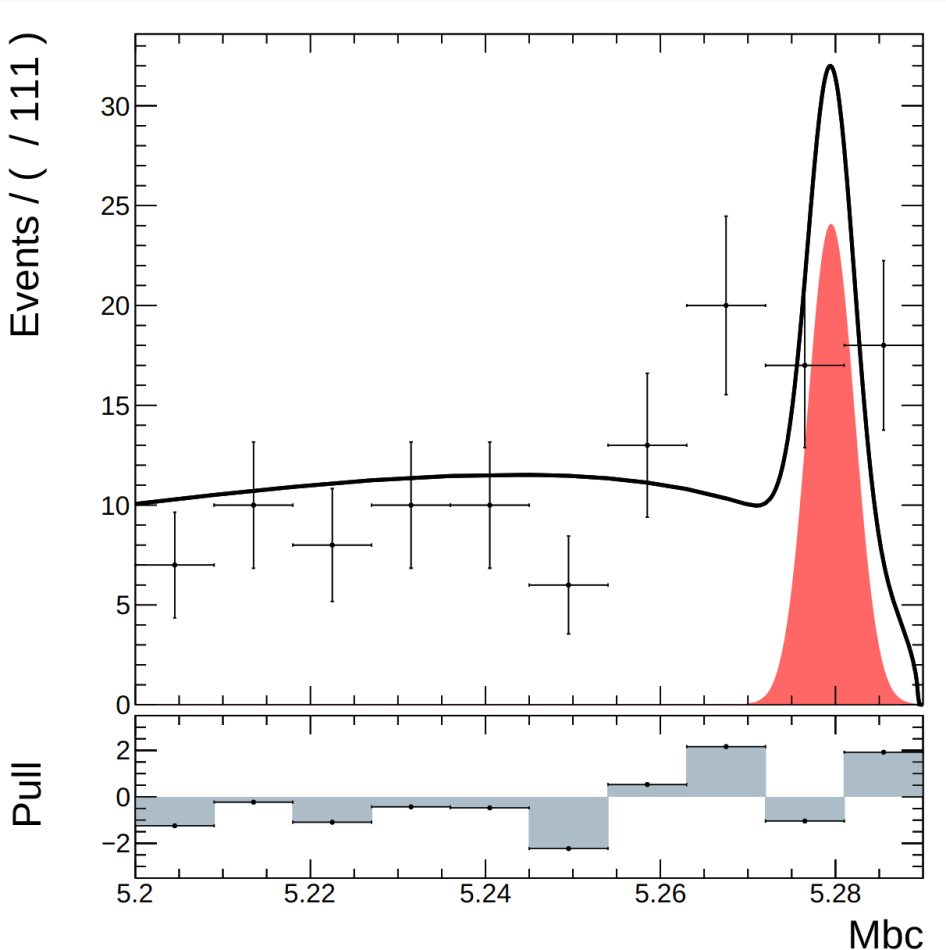
\includegraphics[height=5cm]{figures/mbc-hist-2d-data}
		\label{}
	\end{minipage}
	\begin{minipage}[b]{0.5\linewidth}
		\centering 
		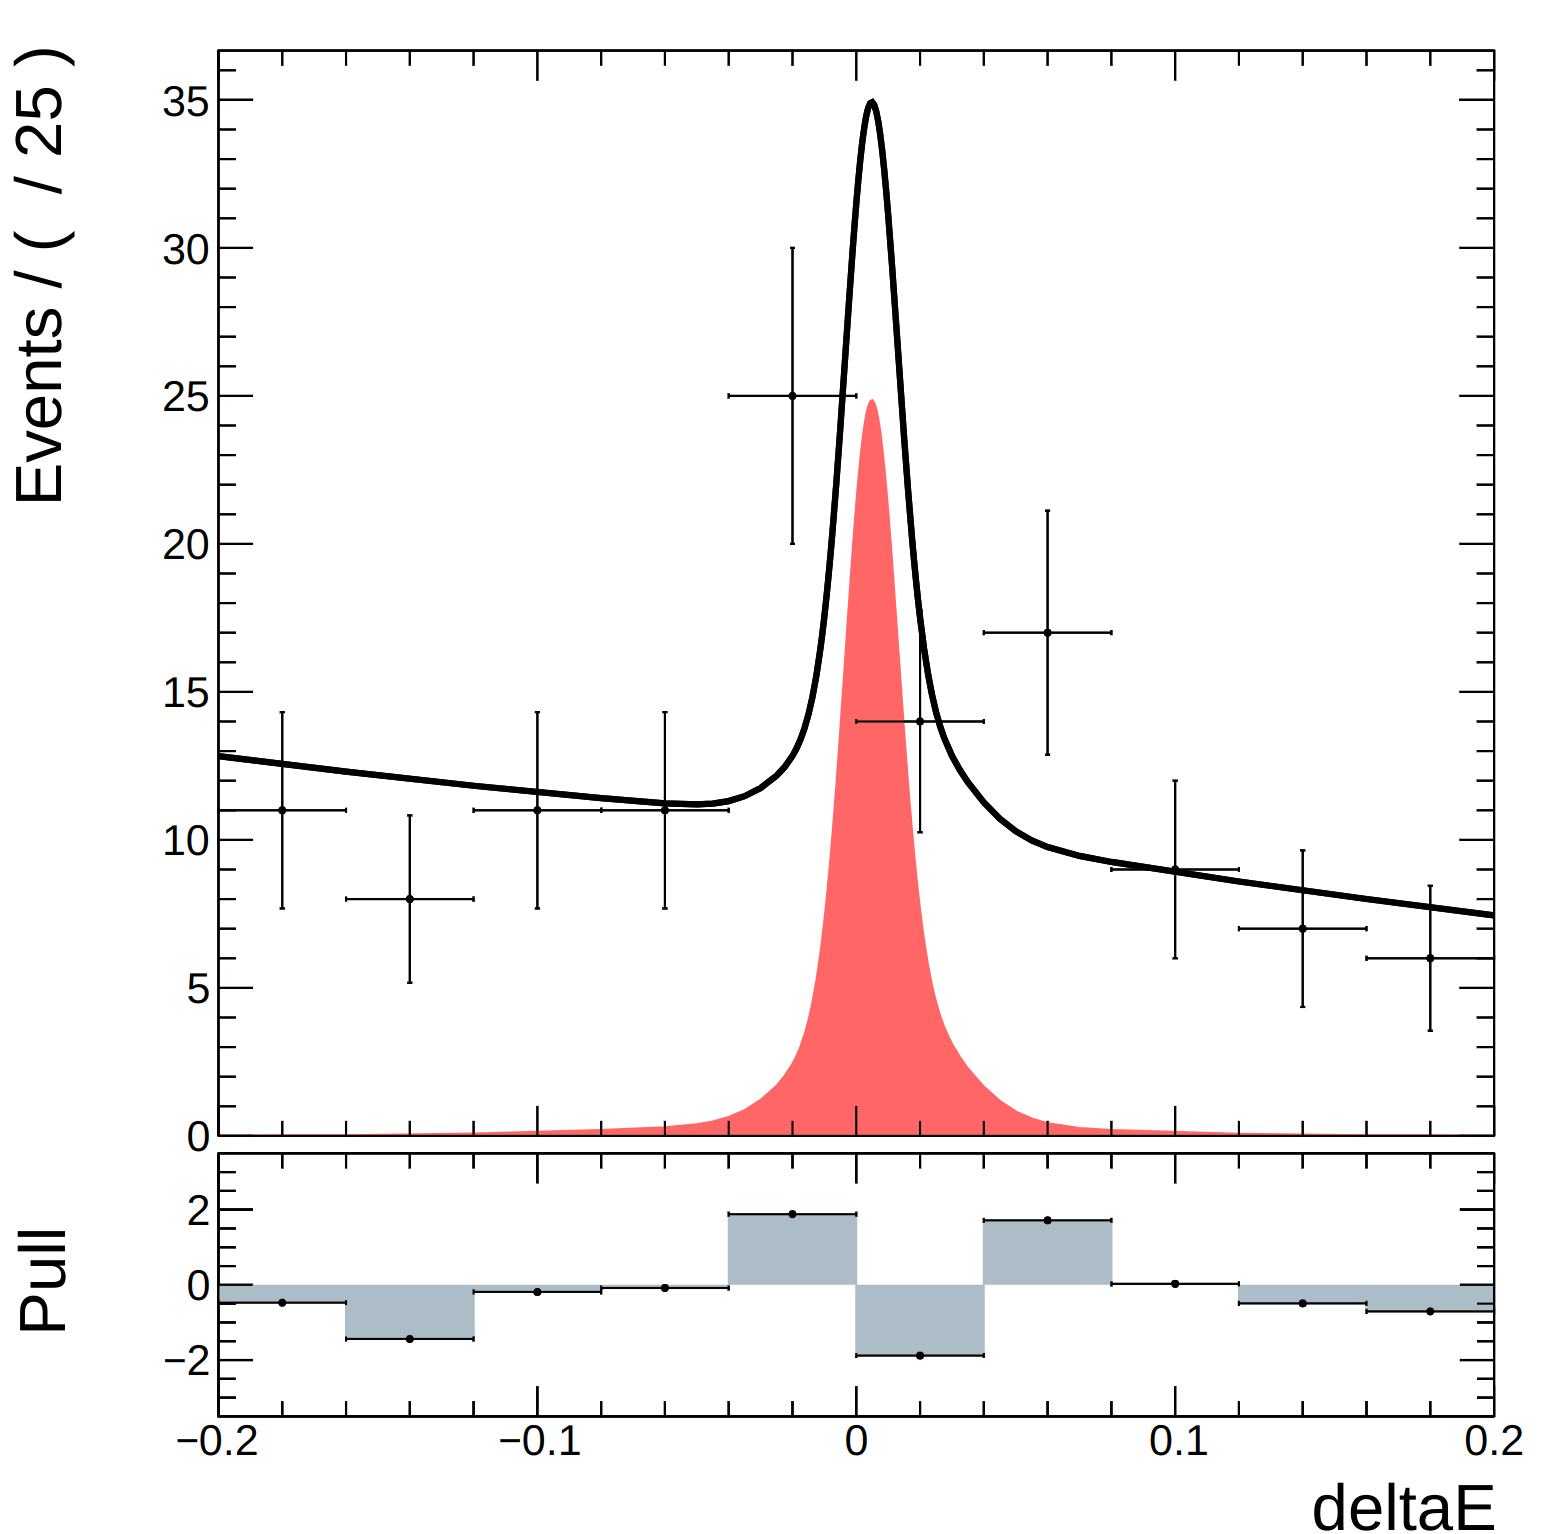
\includegraphics[height=5.2cm]{figures/dE-hist-2d-data}
		\label{}
	\end{minipage}
\begin{minipage}[b]{0.5\linewidth}
	\centering 
	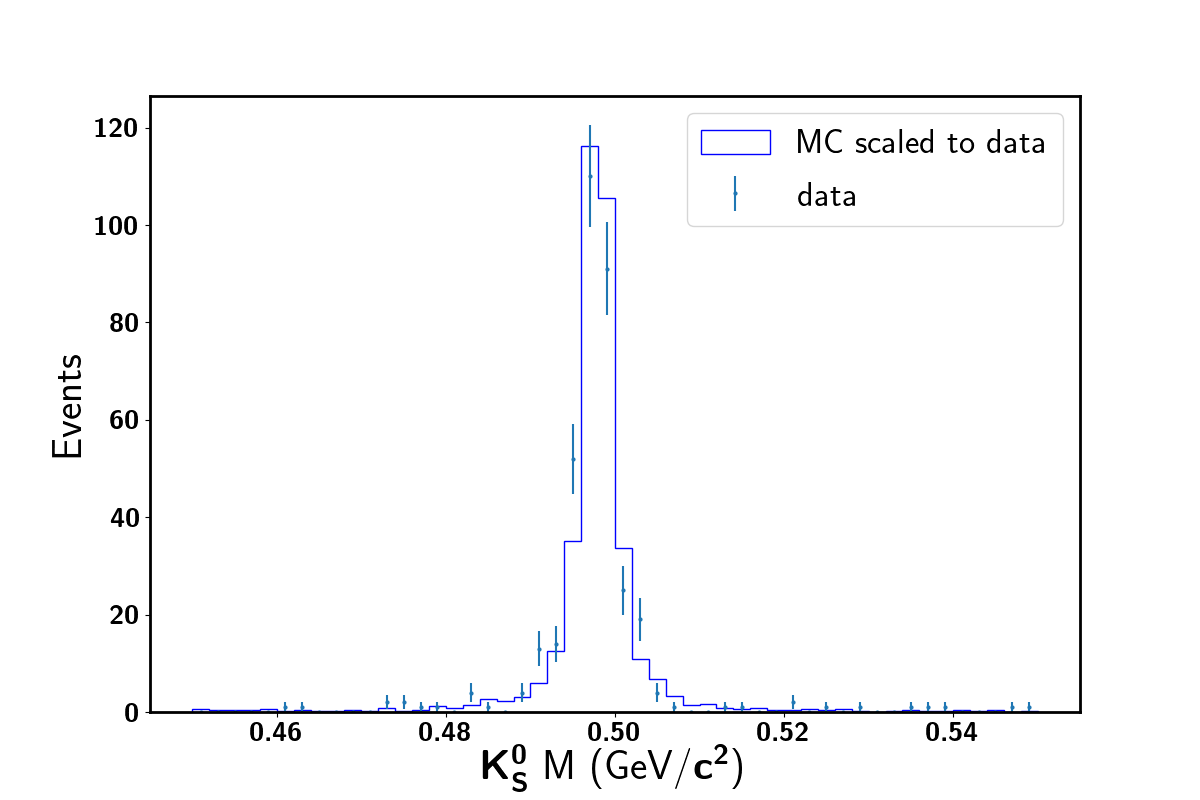
\includegraphics[height=6cm]{figures/best_KsM}	
\end{minipage}
\begin{minipage}[b]{0.5\linewidth}
	\centering 
	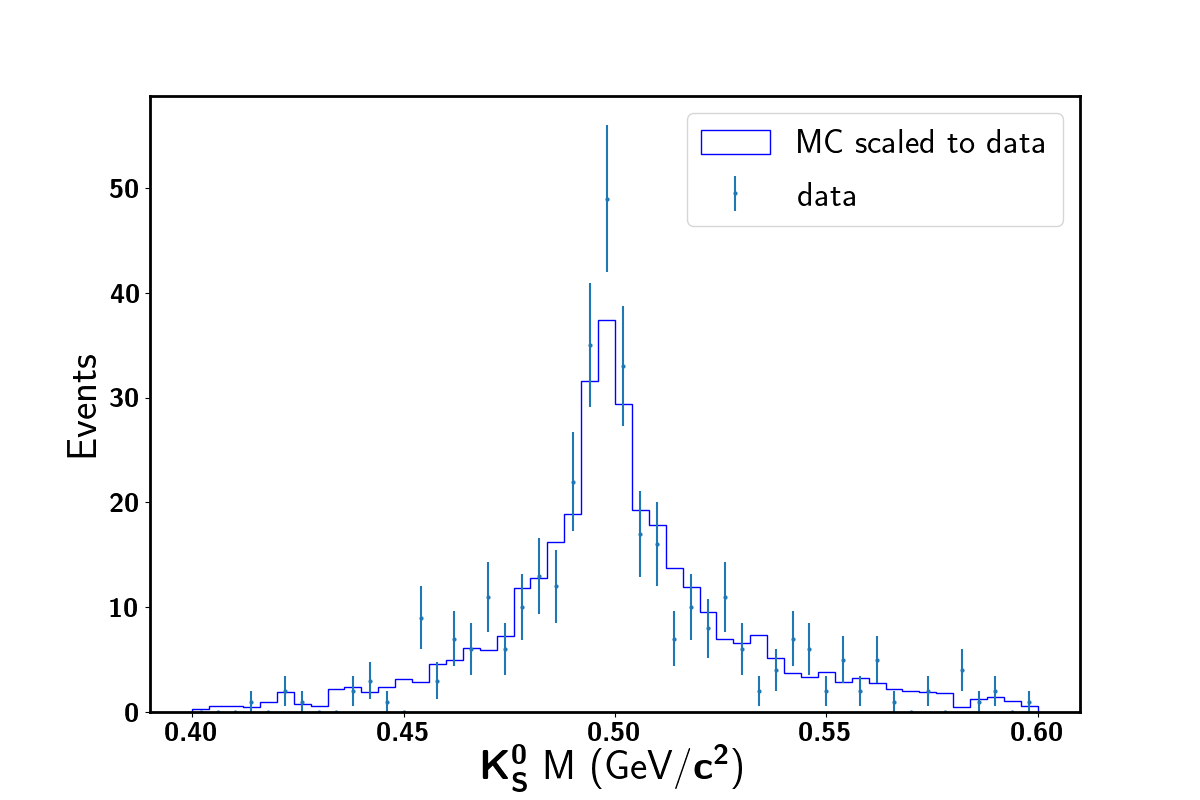
\includegraphics[height=6cm]{figures/best_KsInvM}	
\end{minipage}
\caption{Top: $M_{bc}$ and $\Delta E$ 2D fit using 62.8 fb$^{-1}$data, the red is signal PDF.
	Bottom: ``M" and ``InvM" from data and generic MC which is scaled to data luminosity. The distributions is in a reasonable consistency. }
\end{figure}
 The number of signal events is extracted by integral of fit function over the signal region which is defined as $5.27 < M_{bc} < 5.29 $ GeV and $-0.1 < \Delta E < 0.1$ GeV.
 The expected signal events with ~35\% efficiency in this analysis is calculated as:
 \begin{equation}
 \mathcal{B}(B^0 \to K_S^0  K_S^0  K_S^0)=
 \frac{N_{sig}}{\mathcal{B}(K_S^0\to \pi^+\pi^-)^3\times
 	\epsilon_{rec}\times N_{B\bar{B}}}
 \end{equation}
 In 1 ab$^{-1}$ generic MC13, $7.7\times 10^8 \times 6\times 10^{-6}(BR:B^0\to3K_S^0) \times 21\%(BR:K_S^0\to \pi^+\pi^-) \times 35\% \simeq 339$. The fit result from $M_{bc}$/$\Delta E$ yields $341\pm 20$ events which agrees with expectation. The event number in sideband $M_{bc}<5.26$ GeV in generic MC is 507. Compared to Belle result with $772\times 10^6$ $B\overline{B}$ pairs used, signal from data yields $327\pm 19$, which is also consistent. In 62.8 fb$^{-1}$ data from Belle II, we extract $N_{sig} = 17.4 \pm 4.2$ in this region. Considering the good runs luminosity will be slightly lower than the recorded, the number of signal is in a good agreement with expectation. The sideband region $M_{bc}<5.26$ GeV contains 60 events in data. Both the results of expected event number for signals are consistent in generic MC and data.
To check linearity of the event number fitted from the $M_{bc}$ and $\Delta E$ in this low statistics case, we extract the fraction of continuum backgrounds from generic MC13 sample rescaled to the experimental data luminosity, which yields about 46.5 background events in 62.8fb$^{-1}$. Then the series of (5,10,15,20,25,30) signal MC13 events is injected into the background, to perform the $M_{bc}$/$\Delta E$ fit to check the output signal events number. The fitted yield from $M_{bc}$/$\Delta E$ shows a good agreement on both signal and background events number in data equivalent luminosity. $M_{bc}$ and $\Delta E$ distribution in each injection test are shown as well. Details about the linearity of signal events are in Fig 4-16.

\begin{figure}[H]
	
	\begin{subfigure}{0.5\linewidth}
		\includegraphics[page=1,height=5cm]{figures/injection_sig_5/ds_gen_Mbc_2D.pdf}
		\caption{signal injected: 5}
	\end{subfigure}
	\begin{subfigure}{0.5\linewidth}
		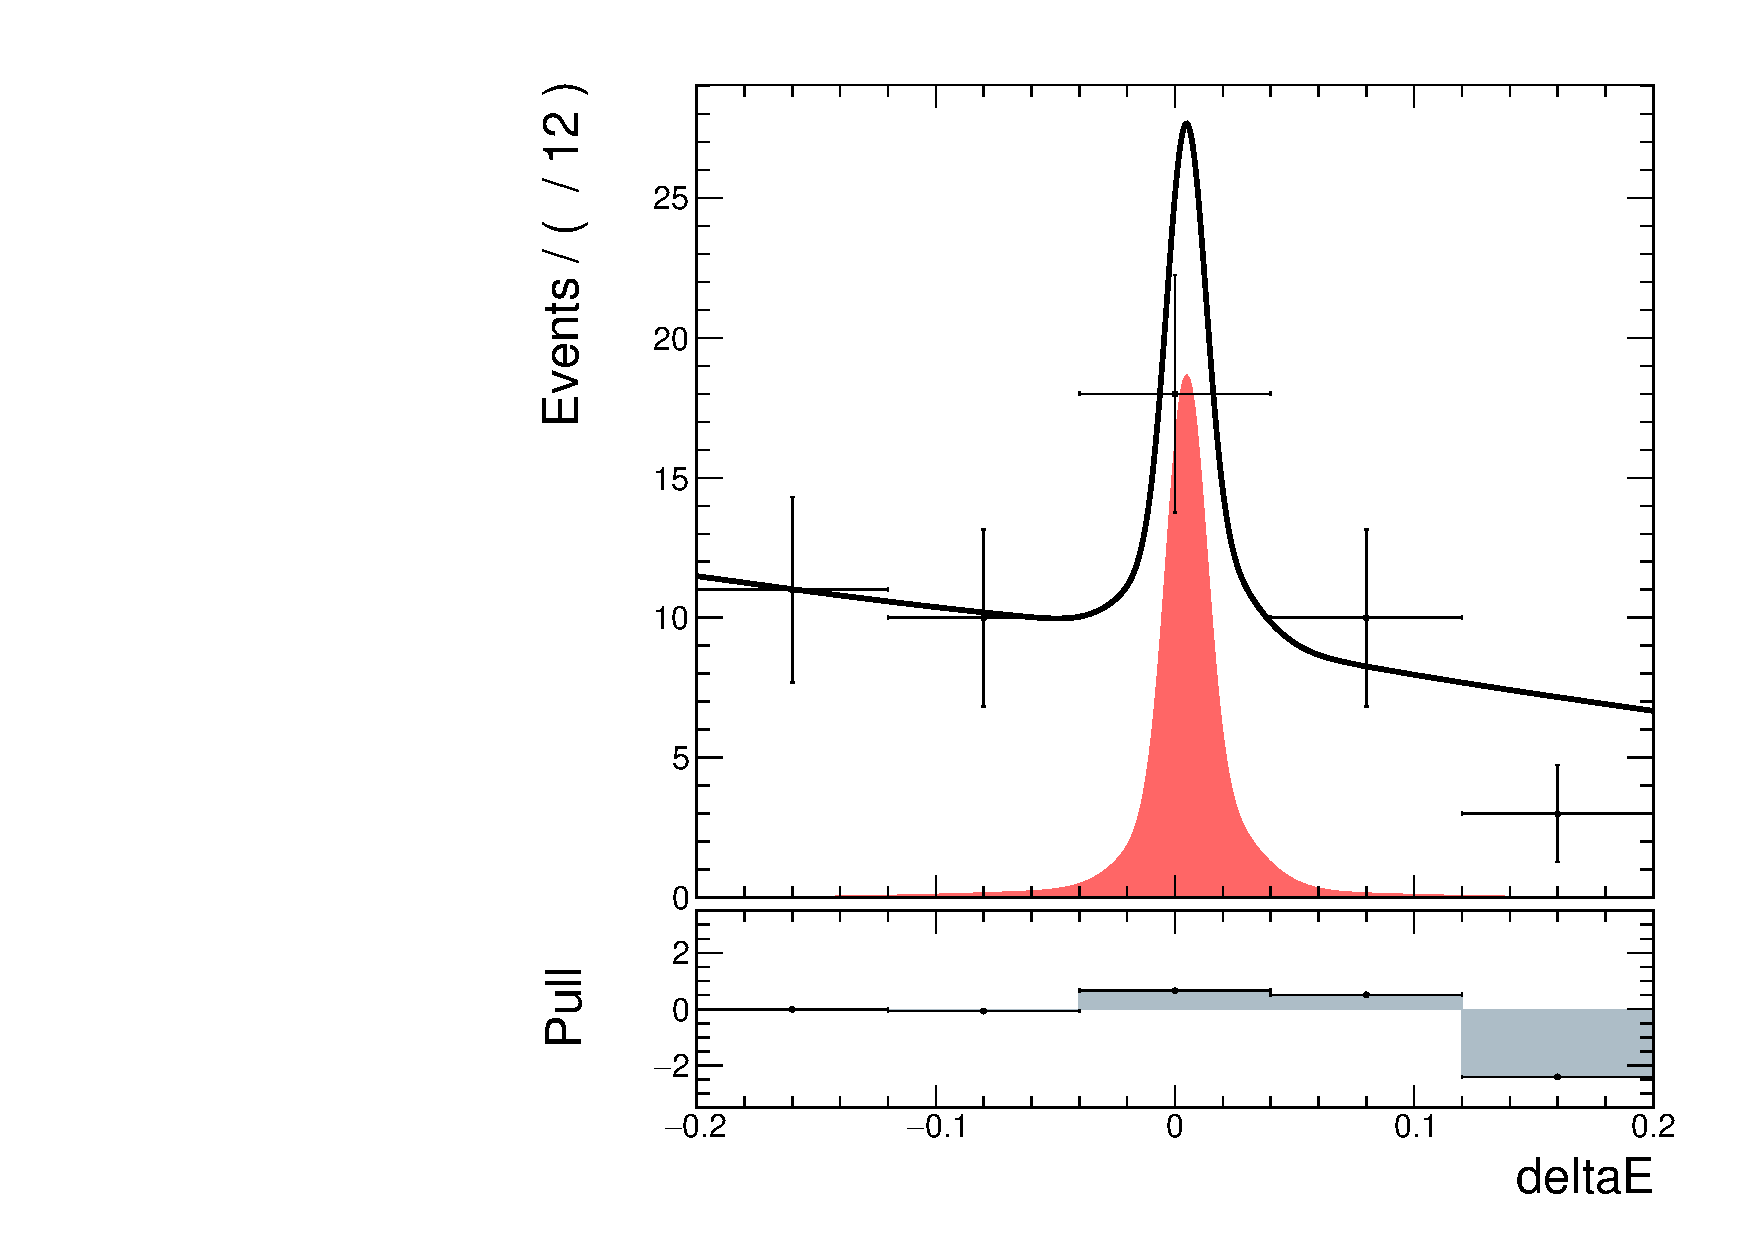
\includegraphics[page=1,height=5cm]{figures/injection_sig_5/ds_gen_deltaE_2D.pdf}
		\caption{signal injected: 5}
	\end{subfigure}
	\begin{subfigure}{0.5\linewidth}
		\includegraphics[page=1,height=5cm]{figures/injection_sig_10/ds_gen_Mbc_2D.pdf}
		\caption{signal injected: 10}
	\end{subfigure}
	\begin{subfigure}{0.5\linewidth}
		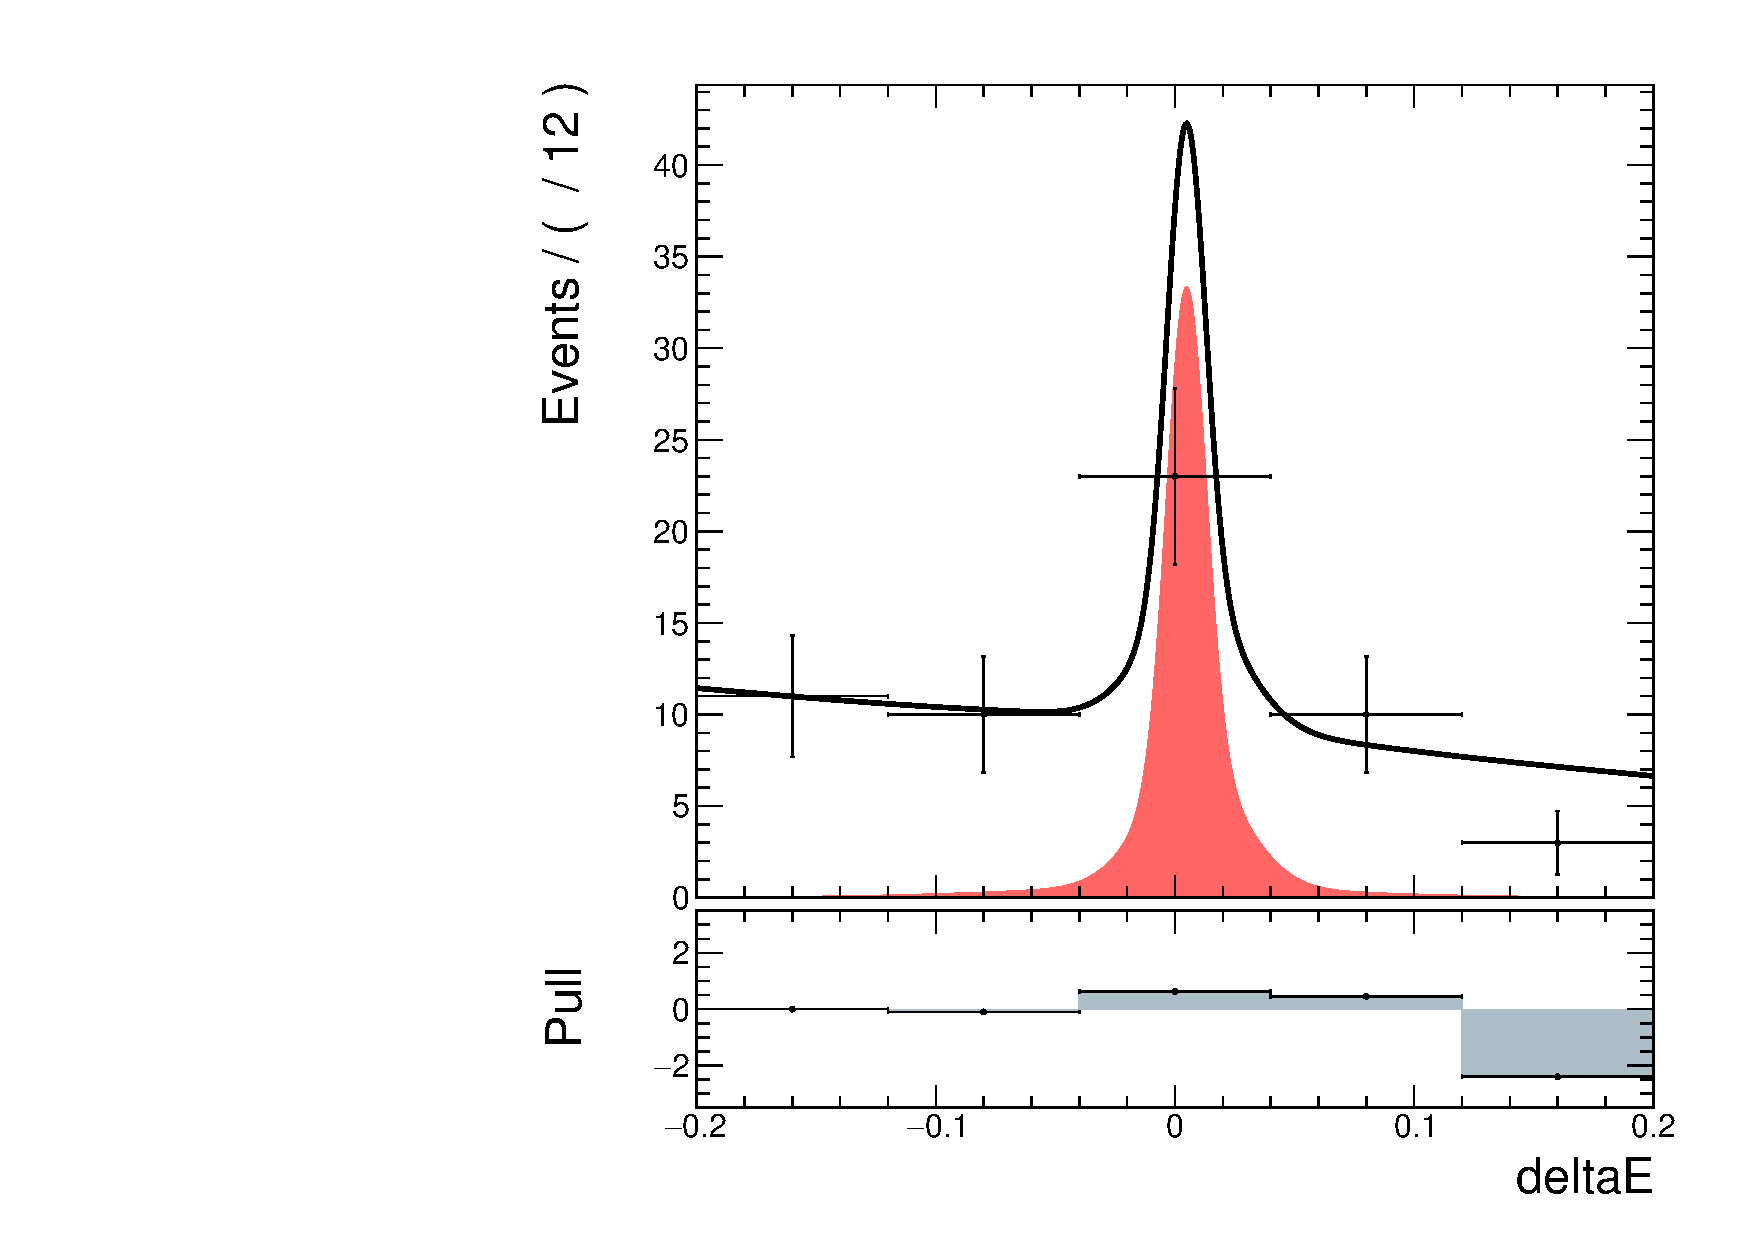
\includegraphics[page=1,height=5cm]{figures/injection_sig_10/ds_gen_deltaE_2D.pdf}
		\caption{signal injected: 10}
	\end{subfigure}
	\begin{subfigure}{0.5\linewidth}
		\includegraphics[page=1,height=5cm]{figures/injection_sig_15/ds_gen_Mbc_2D.pdf}
		\caption{signal injected: 15}
	\end{subfigure}
	\begin{subfigure}{0.5\linewidth}
		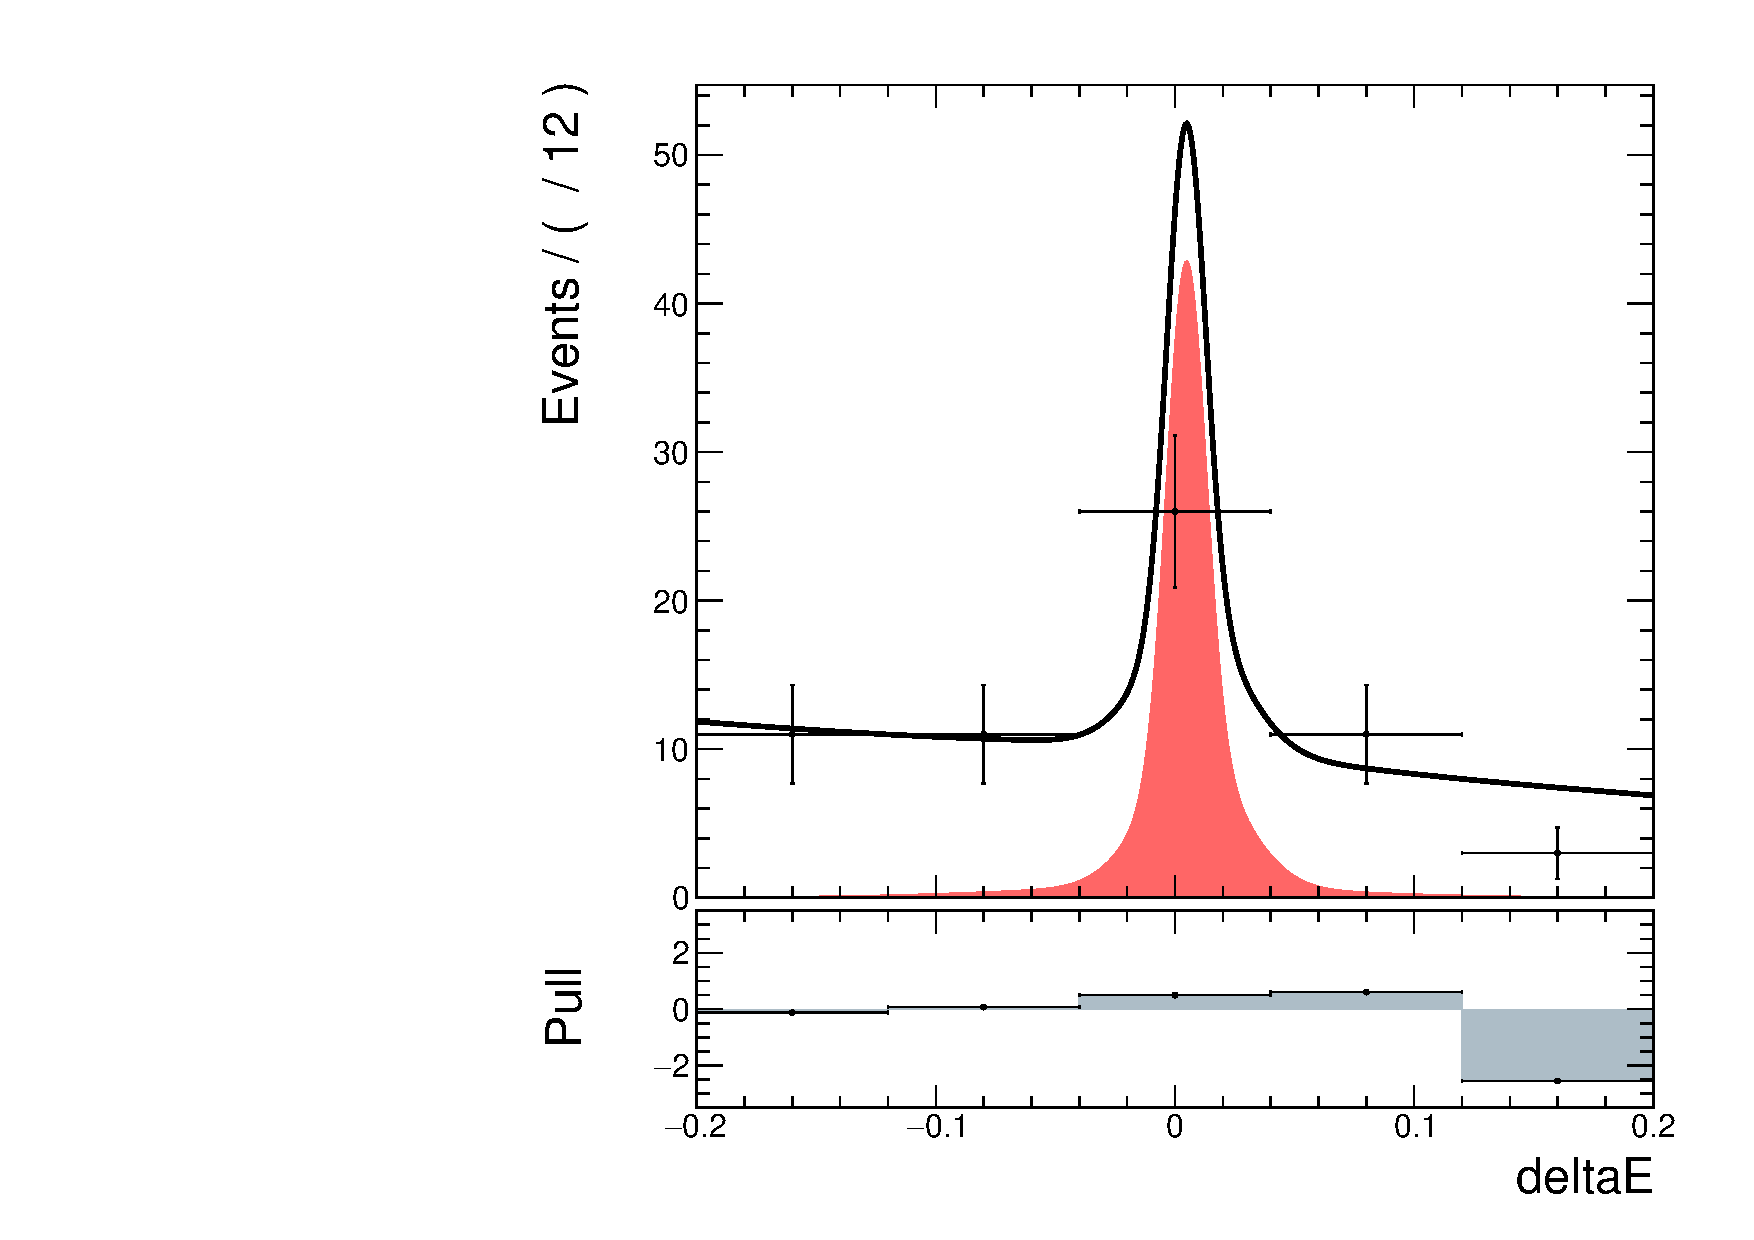
\includegraphics[page=1,height=5cm]{figures/injection_sig_15/ds_gen_deltaE_2D.pdf}
		\caption{signal injected: 15}
	\end{subfigure}
\end{figure}

\begin{figure}[H]
	\ContinuedFloat
	\begin{subfigure}{0.5\linewidth}
		\includegraphics[page=1,height=5cm]{figures/injection_sig_20/ds_gen_Mbc_2D.pdf}
		\caption{signal injected: 20}
	\end{subfigure}
	\begin{subfigure}{0.5\linewidth}
		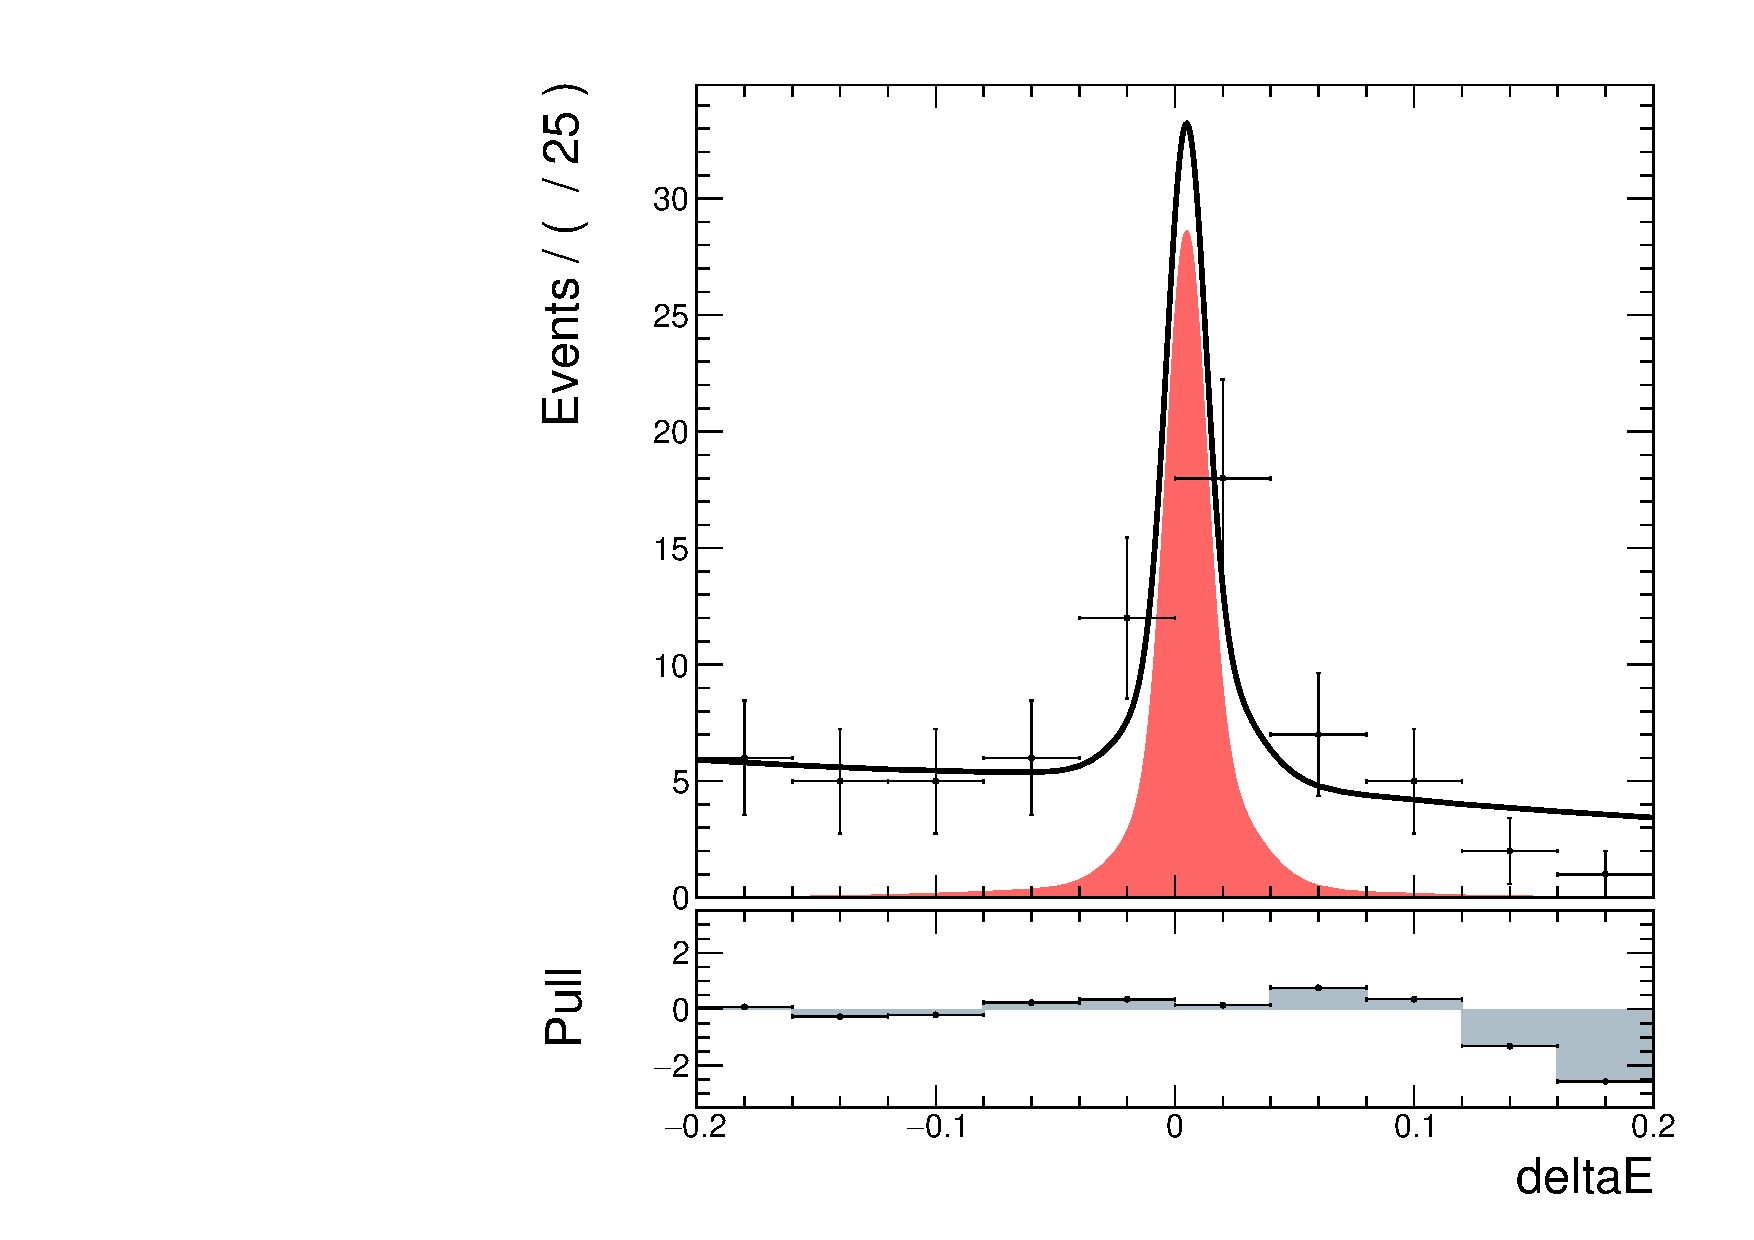
\includegraphics[page=1,height=5cm]{figures/injection_sig_20/ds_gen_deltaE_2D.pdf}
		\caption{signal injected: 20}
	\end{subfigure}
	
	\begin{subfigure}{0.5\linewidth}
		\includegraphics[page=1,height=5cm]{figures/injection_sig_25/ds_gen_Mbc_2D.pdf}
		\caption{signal injected: 25}
	\end{subfigure}
	\begin{subfigure}{0.5\linewidth}
		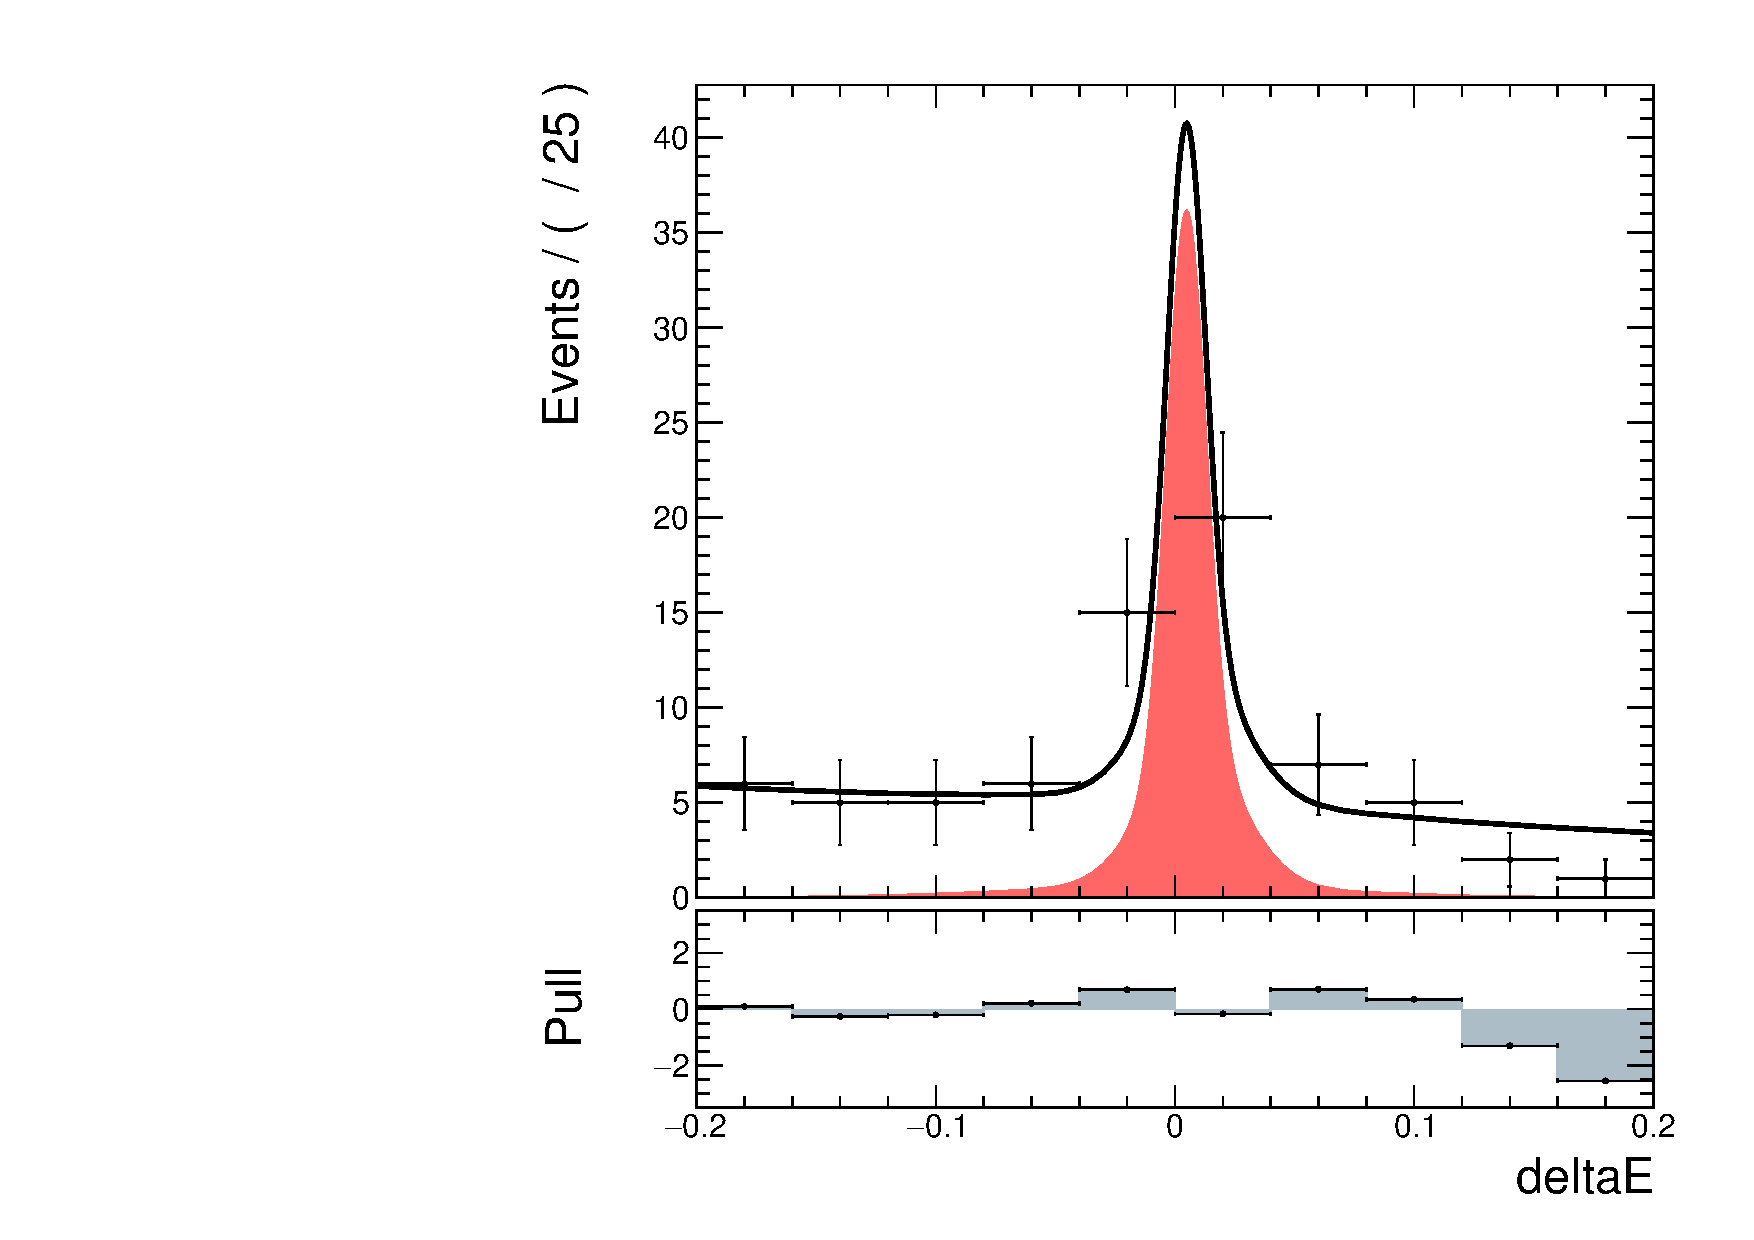
\includegraphics[page=1,height=5cm]{figures/injection_sig_25/ds_gen_deltaE_2D.pdf}
		\caption{signal injected: 25}
	\end{subfigure}
	\begin{subfigure}{0.5\linewidth}
		\includegraphics[page=1,height=5cm]{figures/injection_sig_30/ds_gen_Mbc_2D.pdf}
		\caption{signal injected: 30}
	\end{subfigure}
	\begin{subfigure}{0.5\linewidth}
		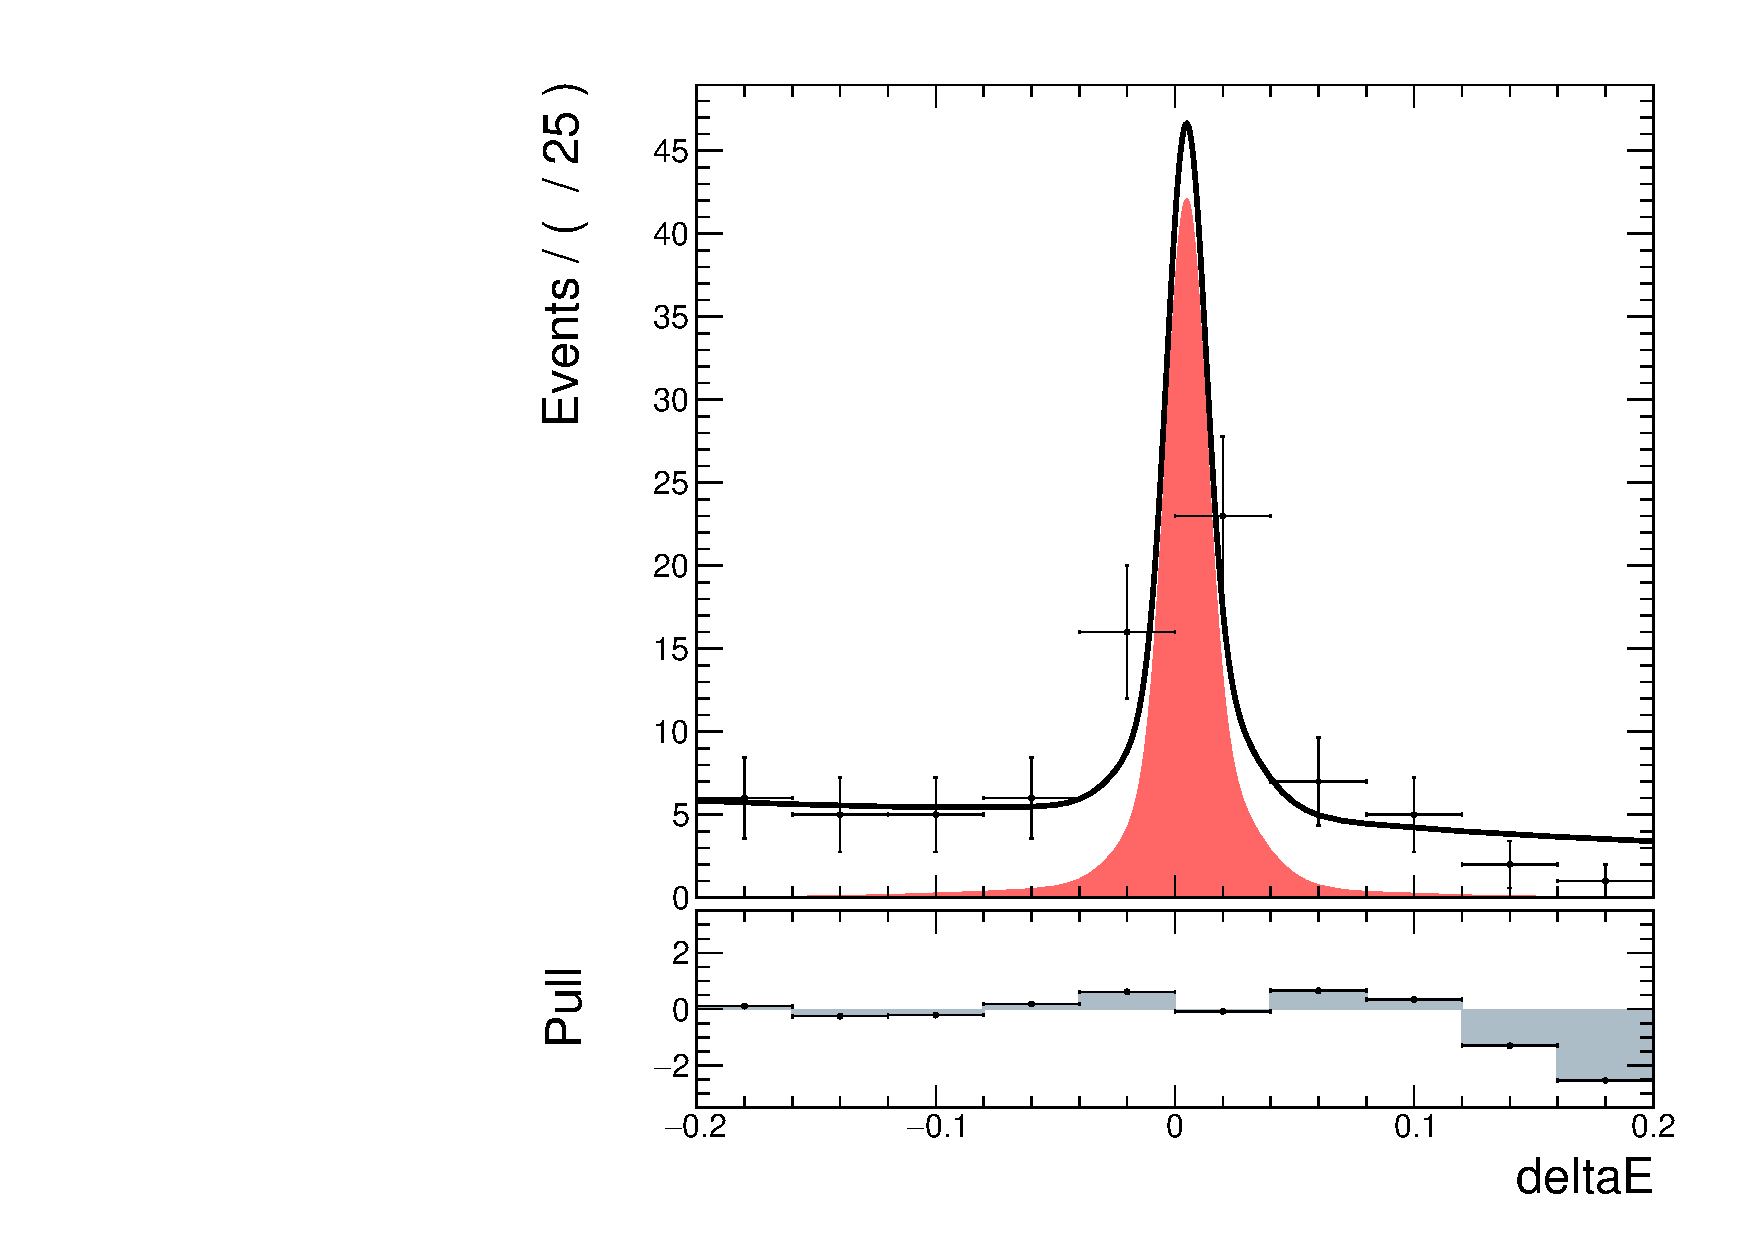
\includegraphics[page=1,height=5cm]{figures/injection_sig_30/ds_gen_deltaE_2D.pdf}
		\caption{signal injected: 30}
	\end{subfigure}
\end{figure}


\begin{figure}[H]
	\begin{minipage}[b]{0.5\linewidth}
		\centering 
		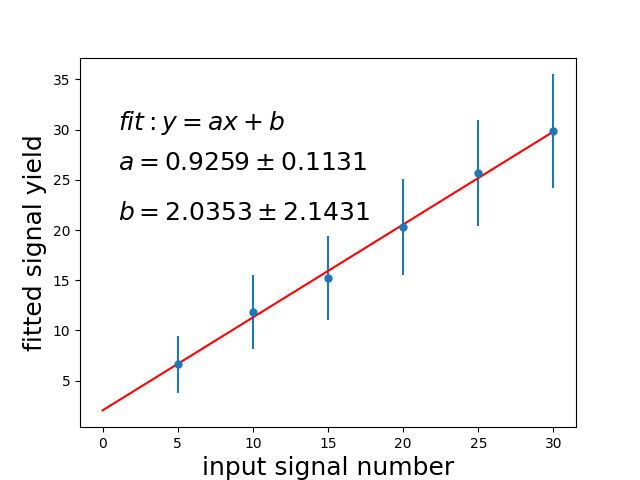
\includegraphics[height=5cm]{figures/inject_line_sig}
		\label{}
	\end{minipage}
	\begin{minipage}[b]{0.5\linewidth}
		\centering 
		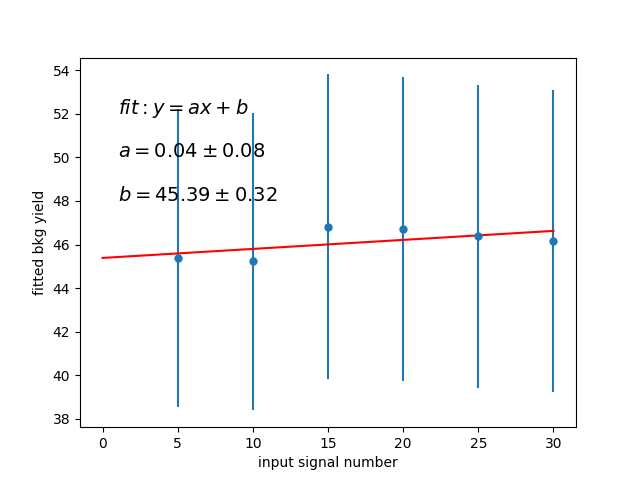
\includegraphics[height=5.2cm]{figures/inject_line_bkg}
		\label{}
	\end{minipage}
	\caption{Injection test for signal extraction. The linearity is clear between input and output signal events number.}
\end{figure}

\begin{comment}
\begin{figure}[htpb]
\centering 
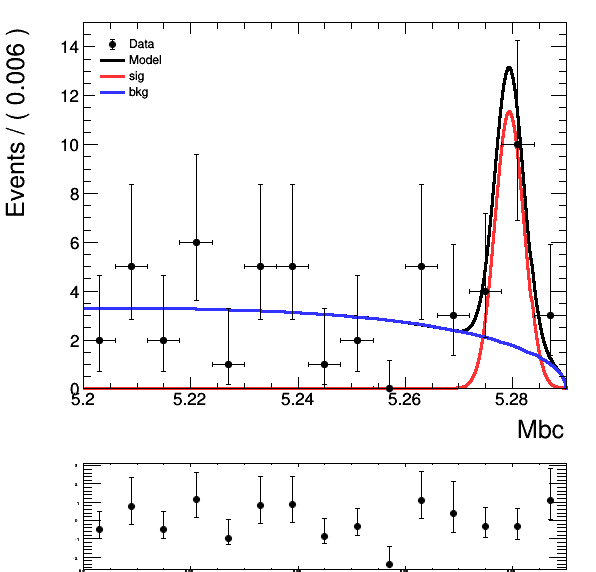
\includegraphics[width=0.7\linewidth]{data-mbc-fit}
\caption{$M_{bc}$ fit in data, signal is Gaussian and background is Argus.}
\end{figure}
\begin{figure}[htpb]
\centering 
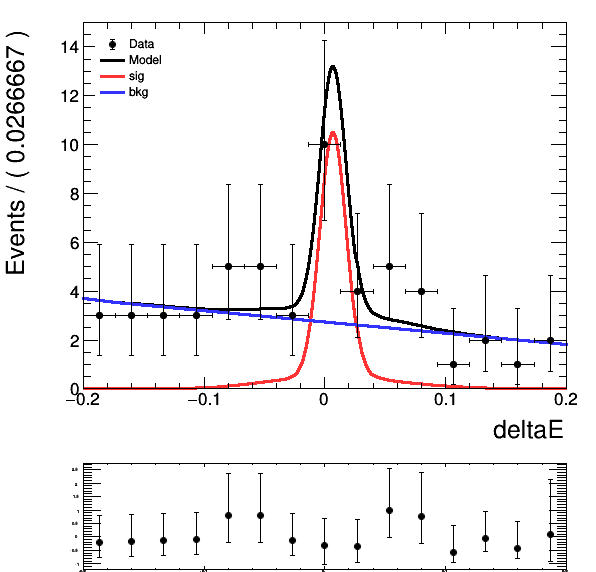
\includegraphics[width=0.7\linewidth]{data-dE-fit}
\caption{$\Delta{E}$ fit in data, signal is double-Gaussian and background is Chebyshev polynomial.}
\end{figure}
\begin{table}[htpb]
\centering
\caption{Fit results from RooFit on $M_{bc}$ and $\Delta E$}
\begin{tabular}{|c|c|c|}
\hline
Floating Parameters  & Mean Value & +/- Error  \\
\hline
N\_sig & 12.8 & 3.93\\
\hline
N\_bkg  & 41.2 & 6.62 \\
\hline
a0 & -0.34 & 0.264\\
\hline
$\chi_{argus}$ & -15.0 & 16.7\\
\hline
\end{tabular}
\end{table}

The fraction of signal and background can be obtained by integral over signal box region using 2D P.D.F. We define signal box using signal MC distribution in Fig 4.13 and 4.14, which $5.269 < M_{bc} < 5.287$ GeV and $-0.09 < \Delta E < 0.12$ GeV. The results are: 

\begin{eqnarray}
N_{sigbox} = 12.6 \pm 3.9\\
N_{bkgbox} = 2.6 \pm 0.2 
\end{eqnarray}

Compared with Belle experience, which similar analysis is done by using about 1$ab^{-1}$ data, signal yield is $327.1 \pm 19.4$. The estimated branching fraction of $B^0 \to K_S^0  K_S^0  K_S^0$ is: 
\end{comment}


\subsection{Kinematics and Vertexing Dependence on KsFinder} 

KsFinder largely reduce the combinatorial background of $B^0$. The previous section shows a good reconstruction performance at low statistics in early phase 3 data. Without the power of rejection provided by $K_S^0$ finder, rediscovery of $B^0 \to K_S^0  K_S^0  K_S^0$ in early phase 3 of Belle II won't be feasible. 
\begin{comment}
\begin{figure}[htpb]
\centering
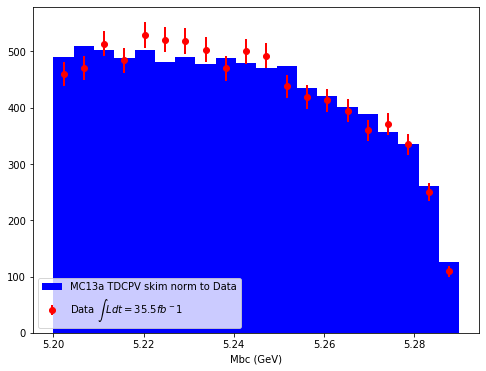
\includegraphics[width=0.7\linewidth]{mbc-noks}
\caption{$M_{bc}$ distribution in data(red) and MC(blue) without $K_S^0$ finder}
\end{figure}
\begin{figure}[htpb]
\centering
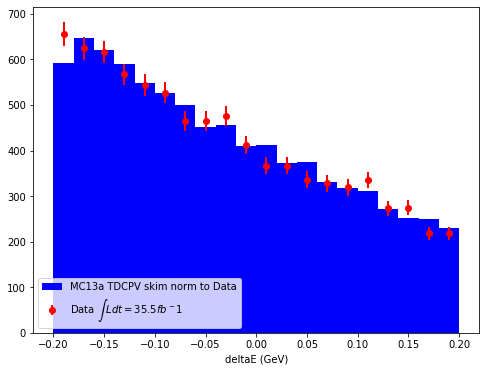
\includegraphics[width=0.7\linewidth]{dE-noks}
\caption{$\Delta{E}$ distribution in data(red) and MC(blue) without $K_S^0$ finder}
\end{figure}
\end{comment}

 However, it's essential to check the potential impact on kinematics and vertexing of $K_S^0$ regarding the implementation of KsFinder. The $K_S^0$ classification uses information such as invariant mass and decay vertex which may propagate bias into $B^0$ vertexing, eventually may affect $\it{CP}$ parameters. Besides, kinematics bias might tune the shape of fit function and contribute bias in defining signal fraction used in \textit{CP} fit. At last, since we have different types of $K_S^0$ based on their SVD hit numbers, a check with $B^0$ based on different $K_S^0$ types are also worthy of doing.
 
 Given each type of $B^0$ based on how many CDC-only tracks it has in final states, the check on $M_{bc}$ and $\Delta{E}$ with or without KsFinder is done by fitting the distribution in signal. $M_{bc}$ and $\Delta{E}$ are modeled by double-Gaussian. Compared corresponding fit results, no clear bias on $M_{bc}$ and $\Delta{E}$ are found by using KsFinder or not. Results are plotted in Fig 4-17 and 4-18. The main distribution of $M_{bc}$ and $\Delta E$ show very trivial difference. 
 \begin{figure}[htpb]
 	\centering
 	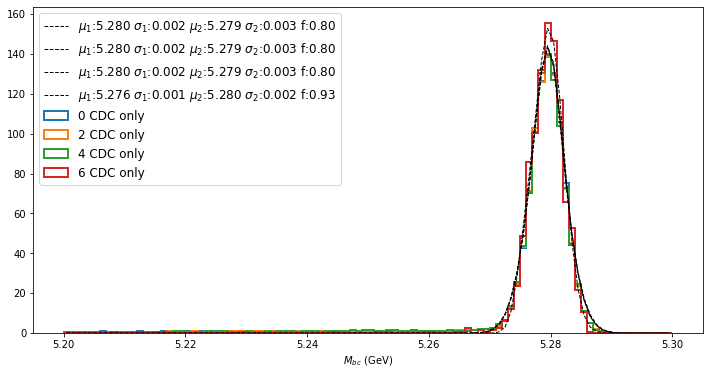
\includegraphics[width=0.7\linewidth]{bias-mbc}
 	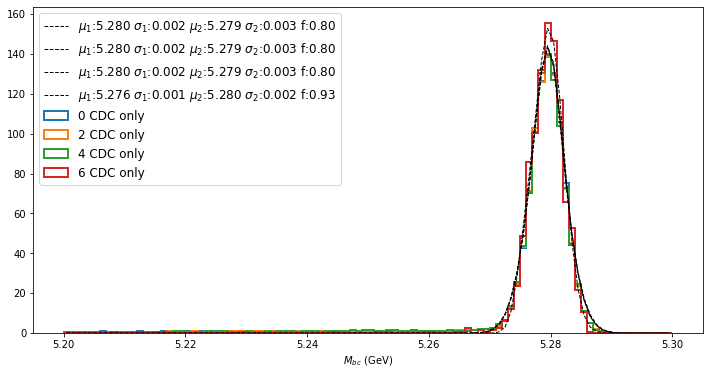
\includegraphics[width=0.7\linewidth]{bias-mbc-ks}
 	\caption{$M_{bc}$ distribution based number of CDC-only tracks in final states. Up: no $K_S^0$ finder; Down: $K_S^0$ finder used.  f is the fraction for the first Gaussian}
 \end{figure}
 \begin{figure}[htpb]
	\centering
	\includegraphics[width=0.7\linewidth]{bias-de}
	\includegraphics[width=0.7\linewidth]{bias-de-ks}
	\caption{$\Delta{E}$ distribution based number of CDC-only tracks in final states. Up: no $K_S^0$ finder; Down: $K_S^0$ finder used. f is the fraction for the first Gaussian}
\end{figure}

Similar to the comparison of $M_{bc}$ and $\Delta{E}$, Z direction vertex position along with its uncertainties are also checked. No clear bias on vertex position and uncertainties are spotted either. Results are plotted in Fig 4.19 and 4.20. And it obivious that the resolution of vertex on z-axis is much worse when the final states of $B^0$ only have CDC tracks. 

\begin{figure}[htpb]
	\centering
	\includegraphics[width=0.7\linewidth]{bias-z}
	\includegraphics[width=0.7\linewidth]{bias-z-ks}
	\caption{$\Delta z$ distribution based number of CDC-only tracks in final states. Up: no $K_S^0$ finder; Down: $K_S^0$ finder used. f is the fraction for the first Gaussian}
\end{figure}
\begin{figure}[htpb]
	\centering
	\includegraphics[width=0.7\linewidth]{bias-zerr}
	\includegraphics[width=0.7\linewidth]{bias-zerr-ks}
	\caption{$\delta\Delta z$ distribution based number of CDC-only tracks in final states. Up: no $K_S^0$ finder; Down: $K_S^0$ finder used.}
\end{figure}
Above all, no clear sign of bias on both kinematics and vertex position from using $K_S^0$ finder has been found, KsFinder implements a small shift on the vertex positions which is trivial compared to the large statistical uncertainty. For the moment, there's no correction on these variables are considered based on the neglect able difference from using KsFinder. And further effects will be watched in future improvement of KsFinder.

\subsection{Summary}
To properly reconstruct $B^0$, a typical cut-based loose selection of $K_S^0$ is first done and then developed KsFinder using FastBDT classification is applied. Due to the tracking issue regarding the $K_S^0$ daughters missing SVD hits, fit mass with varied cuts are used in addition. Combining $K_S^0$ candidates and implementing continuum suppression from event-shape analysis yield signal $B^0$ with relatively low background in full range. 2D fit on $M_{bc}$ and $\Delta{E}$ are performed to extract signal and background number inside defined signal box. The results are in a good agreement in data and MC, as well as Belle result. Potential data MC correction of using KsFinder has been studied. The potential bias on kinematics and vertexing are also studied, which are in a trivial level under the current luminosity.
